%template taken from
%University of Bonn Master of Life Science Informatics
% arara: pdflatex: { synctex: on }

\documentclass[twoside, 12pt,  footinclude=true,  headinclude=true,  cleardoublepage=empty]{scrbook}

\usepackage[utf8]{inputenc}
\usepackage [english] {babel}


\usepackage[
backend=biber,
style=alphabetic,
citestyle=authoryear
]{biblatex}
\addbibresource{references.bib}

\usepackage{lipsum}
\usepackage[linedheaders,parts,pdfspacing]{classicthesis}
\usepackage{amsmath}
\usepackage{amsthm}
\usepackage{booktabs}
\usepackage{graphicx}
\usepackage{float}
\usepackage{indentfirst}
\usepackage [T1]{fontenc}
\usepackage{listings}
\usepackage{color}
\usepackage{multirow}
\usepackage{tikz}
\usepackage[toc,page]{appendix}
\usepackage{MnSymbol}
\usepackage{longtable}
\usepackage{graphicx}
\usepackage{subcaption}
\usepackage{mathtools}
\usepackage{enumerate}
\usepackage{csquotes}
\usepackage{amsmath}
\usepackage{hyperref}
\usepackage{acro}
\usepackage[a4paper,includeall,bindingoffset=20mm,margin=2cm,marginparsep=0cm,marginparwidth=0cm]{geometry}
\usepackage[font={footnotesize,it}, labelfont=bf]{caption}

\setlength{\parskip}{1em}

\DeclareAcronym{AD}{
	short = AD ,
	long  = Alzheimer's disease
}
\DeclareAcronym{API}{
	short = API ,
	long  = Application Programming Interface
}
\DeclareAcronym{BioPAX}{
	short = BioPAX,
	long  = Biological Pathway Exchange Language
}
\DeclareAcronym{BEL}{
	short = BEL,
	long  = Biological Expression Language
}
\DeclareAcronym{BELIEF}{
	short = BELIEF,
	long  = Biological Expression Language Information Extraction Workflow
}
\DeclareAcronym{BRENDA}{
	short = BRENDA,
	long  = Braunschweig Enzyme Database
}
\DeclareAcronym{ChEBI}{
	short = ChEBI,
	long  = Chemical Entities of Biological Interest
}
\DeclareAcronym{CI}{
	short = CI,
	long  = Continuous Integration
}
\DeclareAcronym{CSV}{
	short = CSV,
	long  = Comma Separated Values
}
\DeclareAcronym{DL}{
	short = DL,
	long  = Descriptive Logic
}
\DeclareAcronym{eQTL}{
	short = eQTL,
	long  = Expression Quantitative Trait Loci
}
\DeclareAcronym{eSNPO}{
	short = eSNPO,
	long  = eQTL Single Nucleotide Polymorphism Ontology
}
\DeclareAcronym{FCS}{
	short = FCS,
	long  = Functional Class Scoring
}
\DeclareAcronym{GML}{
	short = GML,
	long  = Graph Markup Language
}
\DeclareAcronym{GO}{
	short = GO,
	long  = Gene Ontology
}
\DeclareAcronym{GraphQL}{
	short = GraphQL,
	long  = Graph Query Language
}
\DeclareAcronym{GRP}{
	short = GRP,
	long  = Gene Set File Format
}
\DeclareAcronym{GSEA}{
	short = GSEA,
	long  = Gene Set Enrichment Analysis
}
\DeclareAcronym{HGNC}{
	short = HGNC,
	long  = HUGO Gene Nomenclature Committee
}
\DeclareAcronym{HTML}{
	short = HTML,
	long  = HyperText Markup Language
}
\DeclareAcronym{HUGO}{
	short = HUGO,
	long  = Human Genome Organization
}
\DeclareAcronym{IMI}{
	short = IMI,
	long  = International Medicine Initiative
}
\DeclareAcronym{INDRA}{
	short = INDRA,
	long  = Integrated Dynamical Reasoner and Assembler
}
\DeclareAcronym{IRI}{
	short = IRI,
	long  = Internationalized Resource Identifier
}
\DeclareAcronym{JGIF}{
	short = JFIG,
	long  = JSON Graph Interchange Format
}
\DeclareAcronym{JSON}{
	short = JSON,
	long  = JavaScript Object Notation
}
\DeclareAcronym{JSONLD}{
	short = JSON-LD,
	long  = JSON Linked Data
}
\DeclareAcronym{KEGG}{
	short = KEGG,
	long  = Kyoto Encyclopedia of Genes and Genomes
}
\DeclareAcronym{MeSH}{
	short = MeSH,
	long  = Medical Subject Headings
}
\DeclareAcronym{NDEx}{
	short = NDEx,
	long  = Network Data Exchange
}
\DeclareAcronym{NeuroMMSig}{
	short = NeuroMMSig,
	long  = Multimodal Mechanistic Signatures for Neurodegenerative Diseases
}
\DeclareAcronym{NPA}{
	short = NPA,
	long  = Network Perturbation Amplitude
}
\DeclareAcronym{OBO}{
	short = OBO,
	long  = Open Biomedical Ontology
}
\DeclareAcronym{OLS}{
	short = OLS,
	long  = Ontology Lookup Service
}
\DeclareAcronym{ORA}{
	short = ORA,
	long  = Over Representation Analysis
}
\DeclareAcronym{OWL}{
	short = OWL,
	long  = Web Ontology Language
}
\DeclareAcronym{PD}{
	short = PD,
	long  = Parkinson's disease
}
\DeclareAcronym{PT}{
	short = PT,
	long  = Pathway Topology
}
\DeclareAcronym{PTSD}{
	short = PTSD,
	long  = Post-traumatic Stress Disorder
}
\DeclareAcronym{miRNA}{
	short = miRNA,
	long  = Micro-Ribonucleic Acid
}
\DeclareAcronym{mRNA}{
	short = mRNA,
	long  = Messenger Ribonucleic Acid
}
\DeclareAcronym{RCR}{
	short = RCR,
	long  = Reverse Causal Reasoning
}
\DeclareAcronym{RDF}{
	short = RDF,
	long  = Resource Description Format
}
\DeclareAcronym{RDFS}{
	short = RDFS,
	long  = Resource Description Format Schema
}
\DeclareAcronym{REST}{
	short = REST,
	long  = Representational State Transfer
}
\DeclareAcronym{RNA}{
	short = RNA,
	long  = Ribonucleic acid
}
\DeclareAcronym{SBML}{
	short = SBML,
	long  = Systems Biology Markup Language
}
\DeclareAcronym{SIF}{
	short = SIF,
	long  = Simple Interaction Format
}
\DeclareAcronym{SPARQL}{
	short = SPARQL,
	long  = SPARQL Protocol and RDF Query Language
}
\DeclareAcronym{SQL}{
	short = SQL,
	long  = Structured Query Language
}
\DeclareAcronym{SNP}{
	short = SNP,
	long  = Single-Nucleotide Polymorphism
}
\DeclareAcronym{SST}{
	short = SST,
	long  = Sampling of Spanning Trees
}
\DeclareAcronym{TBI}{
	short = TBI,
	long  = Traumatic Brain Injury
}
\DeclareAcronym{UBERON}{
	short = UBERON,
	long  = Uber Anatomy Ontology
}
\DeclareAcronym{UniProt}{
	short = UniProt,
	long  = Universal Protein Resource
}
\DeclareAcronym{XML}{
	short = XML,
	long  = eXtensible Markup Language
}
\DeclareAcronym{XMLS}{
	short = XMLS,
	long  = eXtensible Markup Language Schema
}
\DeclareAcronym{XGMML}{
	short = XGMML,
	long  = eXtensible Graph Markup and Modeling Language
}

\title{PhD Thesis}
\author{Andrey Sobolev}
\date{\today}
\begin{document}
	\begin{titlepage}
		\centering
		Bonn-Aachen International Center for Information Technology (B-IT)

		University of Bonn

		 Master Programme in Life Science Informatics

		\vspace{1in}
		 {\Large \bfseries Master's Thesis}
		\vspace{1in}

		{\LARGE \bfseries PyBEL: a Computational Framework for Biological Expression Language}
		\vspace{1in}

		{\large Submitted by}

		{\LARGE Charles Tapley Hoyt\par}

		\vspace{1in}

			First Supervisor: Prof. Dr. Martin Hofmann-Apitius
			\par
			Second Supervisor: Prof. Dr. Thomas Schultz
			\par
			Internal Supervisor: Christian Ebeling

		\vfill
		In collaboration with the Fraunhofer Institute for Algorithms and Scientific Computing (SCAI)
		\begin{flushleft}
			\today
		\end{flushleft}

	\end{titlepage}

%	% Add blank page
%	\newpage
%	\thispagestyle{empty}
%	\mbox{}

	% /frontmatter -> Turn on roman numbering for the following content and turns off normal numbering

	\frontmatter

\chapter*{Acknowledgments}

\begingroup
\setlength{\parskip}{1em}

I would like to sincerely thank my supervisors Prof. Dr. Anton Sirota, Prof. Dr. Christian Leibold and Dr. Kay Thurley for hosting me in the lab, providing help and support for scientific and technical questions. I'd like to thank Dr. Dustin Fetterhoff for his contribution with the recorded data to the project. I'd like to thank Dr. Steffen Katzner for his valuable comments on the project during TAC meetings.

I want to thank the Graduate School of Systemic Neurosciences, led by Prof. Dr. Benedikt Grothe for providing a beautiful and productive atmosphere for students, suitable for networking and discussions.

I would like to specially thank Prof. Dr. Thomas Wachtler, my former supervisor in the German Neuroinformatics Node (G-Node), who supported me in acquiring technical and physiological knowledge required for the current research, during the years of working together in G-Node.

My thanks for the great support from my lab, in particular - Dr. Evgeny Resnik, Fabian Stocek, Dr, Andreas Genewsky, Dr. Elena Itchcovich for their help during surgical procedures, animal handling, data acquisition and analysis.

\endgroup

\tableofcontents

\listoffigures
%\listoftables

\chapter*{Abstract}
Hippocampal cells exhibit preference to be active at a specific place in a familiar environment, enabling them to encode the representation of space within the brain at the population level (\cite{OKEEFE1971171}). These cells rely on the external sensory inputs and self-motion cues, however, it is still not known how exactly these inputs interact to build a stable representation of a certain location (“place field”). Existing studies suggest that both proprioceptive and other idiothetic types of information are continuously integrated to update the self-position (e.g. implementing “path integration”) while other stable sensory cues provide references to update the allocentric position of self and correct it for the collected integration-related errors. It was shown that both allocentric and idiothetic types of information influence positional cell firing, however in most of the studies these inputs were firmly coupled. The use of virtual reality setups (\cite{Thurley2016}) made it possible to separate the influence of vision and proprioception for the price of not keeping natural conditions - the animal is usually head- or body-fixed (\cite{Holscher2005}; \cite{RavassardA.2013}; \cite{Jayakumar2018a}; \cite{Haas2019}), which introduces vestibular motor- and visual- conflicts, providing a bias for space encoding. Here we use the novel CAVE Virtual Reality system for freely-moving rodents (\cite{DelGrosso2018}) that allows to investigate the effect of visual- and positional- (vestibular) manipulation on the hippocampal space code while keeping natural behaving conditions.

In this study, we focus on the dynamic representation of space when the visual-cue-defined and physical-boundary-defined reference frames are in conflict. We confirm the dominance of one reference frame on the other on the level of place fields, when the information about one reference frame is absent (\cite{Gothard2001}). We show that the hippocampal cells form adjacent categories by their input preference - surprisingly, not only that they are being driven either by visual / allocentric information or by the distance to the physical boundaries and path integration, but also by a specific combination of both. We found a large category of units integrating inputs from both allocentric and idiothetic pathways that are able to represent an intermediate position between two reference frames, when they are in conflict. This experimental evidence suggests that most of the place cells are involved in representing both reference frames using a weighted combination of sensory inputs. In line with the studies showing dominance of the more reliable sensory modality (\cite{Jeffery1999}; \cite{Gothard2001}), our data is consistent (although not proving it) with CA1 cells implementing an optimal Bayesian coding given the idiothetic and allocentric inputs with weights inversely proportional to the availability of the input, as proposed for other sensory systems (\cite{Jeffery2016}). This mechanism of weighted sensory integration, consistent with recent dynamic loop models of the hippocampal-entorhinal network (\cite{Li2020}), can contribute to the physiological explanation of Bayesian inference and optimal combination of spatial cues for localization  (\cite{Cheng2007}).


% /frontmatter -> Turn on normal numbering
\mainmatter

\chapter{Introduction}
\label{ch:intro}

\section{Space and navigation as abstract concepts of everyday life}
\label{sec:navig_in_life}

For about a decade I was curious whether reading books from an electronic device is anyhow affecting comprehension or learning, an ability to remember facts, events or their sequence - compared to their paper versions. The modern electronic way of reading exposes many advantages: you can store 1000 books in the same small device, you can quickly search any text by a word, there is an ability to make notes and highlight valuable fragments and, of course, to share all that content between physical devices. These advantages were by far overtaking and convincing towards using electronic versions for reading until I found the research on reading comprehension by \cite{Mangen2013}. They demonstrate that text comprehension was lower for the group of electronic readers, compared to the paper-based readers, and that it is mostly related with the reduced ability to reproduce the sequence of described events for narratives or locating information in texts in general (\cite{GiuliaCataldo2000}). Interestingly, the major hypothesis for the decrease of performance is the reduced spatial representation of the electronic book compared to the printed content (\cite{Mangen2013}). They argue that access to paper texts comes in a coherent combination of visual and tactile cues, allowing a reader to build spatial extension and physical dimension of the text. This is supported by earlier empirical and theoretical studies showing that a good mental spatial representation of the text layout supports reading comprehension (\cite{Kintsch1998}; \cite{PIOLAT1997565}). So building a good spatial representation of the content is important for comprehension and learning.

How else do the abstract concepts of space and navigation have an impact on our life? Let’s jump to the world of classical music and imagine a musical piece. A set of notes (tones) can be taken as a particular music space (e.g. the standard 88 keys on the piano keyboard). A melody, from note to note, accompanied by chords and passages, builds a trajectory in this imaginary music space. This music space has a physical projection called sheet notes, usually printed on paper. While reading sheet notes of a particular piece, we go through the special signs and symbols - “forte” or “piano”, “fermata”, “rest”, “coda” and others, which act as visual cues and landmarks in the current music trajectory. So what is essential to be able to play a music piece? It is inevitable to build a mental representation of the music space in the brain, as well as to be able to navigate in that music space, by learning and executing existing or building new “music” trajectories and linking them to the physical arm and finger actions - depending whether you prefer piano, violin or a guitar (see also “Mental play” in \cite{ChuanChang2016}).

A game of chess is another example of an abstract space, a bit closer to the classical physical “real-world” space representation. The chessboard has its strictly defined boundaries and spatial positions. Direction and type of movements in the chessboard space are predetermined for different actors and also limited depending on the position of other figures. The victory in a game is critically dependent on the ability to build a reliable representation of that chessboard space in the brain, as well as to build a magnitude of possible trajectories that, one after the other, could be implemented by figures of both colors.

Abstract concepts of space and navigation are applicable to many physical modalities. Besides the traditional spatial navigation from a bedroom to a kitchen, from home to work or from Munich to Moscow, we constantly need to solve spatial problems in relative spaces - like to define on which shelf relative to the freezer should I put back a coffee cup, or to imagine somewhere away to the far left in the egocentric space when locating a source of a pleasant sound (see also Buzsáki, 2019, “Space in the world versus space in the brain”). What do all these physical or abstract “spatial” tasks have in common? At the high cognitive level, the implementation of all these types of spatial navigation mostly located in the medial temporal lobe, specifically in the hippocampal-entorhinal system. Having location- and spatial cue-selective neurons (\cite{OKeefe1978}, \cite{Moser2015}), hippocampus and parahippocampal cortex together are able to form representations of not only physical spatial dimensions, but act as a general machinery for building arbitrary representations of physical and abstract spaces (\cite{Aronov2017}). These  mental cognitive maps - dynamic ensembles of cells selective for combinations of physical or abstract spatial features representing unique locations or experiences - are necessary to build and implement navigation in these spaces, potentially via sequential activation of these neural ensembles in a form of mental trajectories (\cite{Hopfield2010}; \cite{Buzsaki2018}).

Up to the moment, the exact mechanisms how these neuronal dynamics are implemented at both  population or single neuron level is still not fully understood. In this work, I’m trying to contribute to the research on navigation in physical space as a special subclass of cognition tasks implemented by the hippocampal-entorhinal system.


\section{Spatial representation in the hippocampal-entorhinal circuit}
\label{sec:spatial_repr}

Spatial navigation in mammals is implemented as a cooperative dynamic neural network, distributed across multiple brain regions. This network encodes not only an allocentric position in space, but also movement direction, as well as the past and future trajectories. The great evidence for it are the discoveries of place cells, grid cells, head direction cells and other types of spatial feature selective cells, located mostly within the hippocampal, parahippocampal and entorhinal brain areas (see review in \cite{Moser2015}). Place cells were defined mostly as neurons selective to a particular location in an environment. Grid cells, one synapse away from the place cells, are also place selective neurons but that are active not at single locations, but at a regularly-spaced intervals, bringing a periodic structure to the physical space inside the cognitive brain map. Place cells are modulated by a variety of inputs, including external visual landmarks, olfactory or tactile cues, translational and rotational signals and integrated proprioceptive signals, which allow them to maintain activity of their place of preference when the sensory signals are absent, like in the absence of light. While place cell activity can unpredictably change from one environment to the next (\cite{Colgin2008}), in contrast, grid cells keep their firing independent of the individual details of a particular environment (\cite{Fyhn2007}), providing a putative metric of space. Additionally, orientation in the environment can be taken from the head-direction system, implemented by the neurons located in different brain areas but importantly in the post-subiculum, and being active when the animal's head is pointed to a certain direction (\cite{Taube2007}). More specific cell types, like boundary-vector cells, or cells responding to a combination of environmental features (\cite{Deshmukh2013}; \cite{Hooydal2019}) extend the navigation system in fine-tuning actual position estimation, in correcting accumulated positional errors and perfecting future spatial planning. Below, there is a short review of each of the particular cell types and its possible involvement in the brain navigational system. As the exact internal organization of the navigation system is not fully defined yet, at the end of this chapter I discuss open questions and focus on the yet unknown parts of it that I try to address and to make a contribution to in this study.

\subsection{Place cells}

Hippocampal cells responsive to a current location of an animal were first found by O’Keefe and Dostrovsky in 1971. After the discovery, these cells acquired a name of “place cells” (Figure 1a). Although there are many ways of the functional organization in the cortex - like the topographic organization in the visual area V1 (\cite{Schuett2002}), place cells in the CA1 area appeared to not form any simple organizational pattern, such that the neighboring cells may represent different locations and features of the environment. Later it was discovered that the size of the environment, selective for a particular place cell, varies from the cell location within the hippocampus, from dorsal (smaller, precise fields) to ventral (lager fields, \cite{Jung1994}). The emerging interest to the hippocampal research after the place cell discovery led to the discovery of the hippocampal neurons responding to non-spatial features, like odors (\cite{Wood1999}; \cite{Igarashi2014}), border and general tactile information (\cite{Young1994}; \cite{Okeefe1996}), distance or timing (\cite{Hampson1993}; \cite{Kautzky2016}). However, although much of the hippocampal findings relate to the representation of space, it does not limit the role of the hippocampus in declarative memory in general - place representation is just a key element in many episodic or even semantic memories (\cite{Buzsaki2013}).

Importantly, the recordings of hippocampal neurons in novel environments reveal that the majority of place cells appear to have immediate firing fields (\cite{Frank7681}). Although several studies of hippocampal ensembles demonstrate, that often the formation of stable fields takes up to several minutes (\cite{Wilson1993a}), this presence of immediate fields suggests that certain components of the network are pre-wired in the circuit, and that the basic elements (neurons, synaptic connections) of the cognitive map are largely predetermined.
In short summary - place cells provide dynamic and continuous information about the animal’s position in space, and together, on the population level, these cells are able to form a cognitive map - an abstraction in the brain that represents allocentric space.

\begin{figure}
\captionsetup{format=plain}
\makebox[\textwidth]{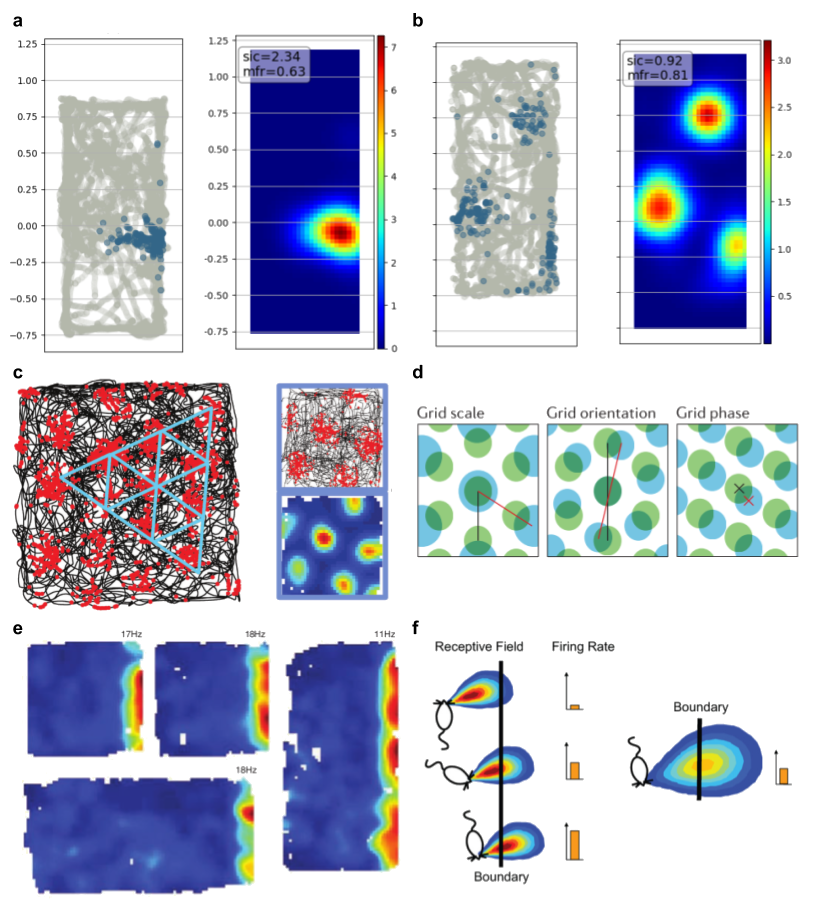
\includegraphics[width=150mm]{figures/F1_place_cells.png}}
\caption[Place and grid cells]{
Place, grid and border cells. \textbf{(a)} Firing rate map of an example hippocampal neuron that is active at a certain location in the rectangular environment - a “place” field. \textbf{(b)} another example neuron that has multiple place fields of different size (examples from the data used in the current study). \textbf{(c)} Firing rate map of an example mEC neuron that is active at certain locations of the environment, that form a hexagonal grid pattern (left). Place preference autocorrelograms reveal hexagonal structure (Adapted with permission from \cite{Moser2015}) \textbf{(d)} Examples of pairs of grid cells having different scale, orientation and phase (adapted with permission from \cite{Moser2014}). \textbf{(e)} Firing rate maps of an example neuron that is active near the right border of the environment, invariant of the environment type (adapted with permission from \cite{Solstad2008}) \textbf{(f)} schematic of the receptive field of an example neuron that is selective for a particular direction and distance to the environmental boundary (\cite{Lever2009}).
}
\label{fig:F1_place_cells}
\end{figure}


\subsection{Grid cells}

In addition to the discovery of the place cells, a few decades after, another important type of the place-selective cells were found in the brain’s entorhinal cortices. Particularly, in the layer II of the Medial Entorhinal Cortex (mEC) neurons, forming discrete regularly spaced firing fields were identified (\cite{Hafting2005}). Surprisingly, the firing fields of those neurons were organized in a grid of tessellating triangles evenly covering the corresponding space (Figure 1c). A simple autocorrelogram analysis revealed the rigid hexagonal structure (Figure 1c right). Key features of the newly discovered cells were, first - their different spacing between individual fields and phase shift relative to each other, with the increasing scale from dorsal to ventral mEC, and second - their anchoring to the boundaries, persistence between environments and independence on visual or olfactory landmarks. These facts suggest this type of cells is primarily based on self-motion and plays a main role in path integration, mixing idiothetic vestibular and proprioceptive signals.
Anatomically, mEC has a direct input to the Hippocampus. This led to the assumption that grid cells, sharing common peak and different spacing, might be a good basis to form place cells, taking grid cell inputs as a linear combination (\cite{OKeefe2005}). However, experimental evidence, based on studies on developing animals, shows that mechanisms are more sophisticated, as there is a delayed maturation of the grid fields relative to place cells. An alternative assumption, that place cells can be formed as a combination of the grid and other cell-type inputs - like border cells (see below), which are ready at the early stages of the development, looked to be more consistent. As suggested (\cite{Savelli2008}), specific place cells may arise as neurons integrating inputs from grid cells that provide proprioceptive-based distance information, and border cells that provide position relative to external boundaries. This putative idiothetic place cells will be named “boundary-driven” or “boundary-vector” cells later in the text.


\subsection{Head direction system}

One of the key components for successful navigation is maintenance of the proper allocentric orientation. Even before grid cells, neurons, which firing rates depend on the animal’s head orientation were found - originally in postsubiculum (\cite{Taube2007}), and later in other nearby areas (mEC, AdN etc.). Besides their primary feature of keeping the absolute directional preference, the “head-direction” cells were shown to maintain their relative directional preferences between each other; however, each cell by itself has no particular preference in absolute world coordinates - its directional preference can change between different environments. Importantly, in absence of light, head direction cells are able to integrate angular velocity of the head and maintain original directional preference, although for the cost of accumulation of directional error.

The presence of head direction cells is a necessary part to perform successful path integration, especially when light or external allocentric sensory cues are not present. The interaction of grid cells, providing distance estimation and a metric for space based on idiothetic inputs, and head direction cells supplying absolute orientation define the basis for position estimation based on path integration, which  is discussed more in one of the next sections of this chapter.


\subsection{Border and BVC cells}

While grid cells and head direction cells provide distance and orientation estimation, respectively, actual position should be estimated in relation to a certain point in space - usually relative to a physical boundary. Further research of the cell functions in the mEC lead to a discovery of the neurons representing geometric boundaries (\cite{Solstad2008}), and cells active at a particular distance to a certain boundary. These “border” and “boundary” cells are active when an animal is located near a certain physical boundary; their firing is independent of affine transformations (Figure 1e). A border cell, or more generally, a putative boundary vector cell (\cite{Barry2006}, \cite{Lever2009}), is another type of the neuronal encoding found in the mEC, that is involved in spatial representation. In a series of recordings these cells demonstrated preference to fire at a certain distance and direction to a particular object (Figure 1f) or, as a special case, to a certain boundary.

Border and boundary-vector cells (BVCs) may play an important role in updating positional signals of grid cells, as the latter tend to drift in open spaces. If the animal hits the boundary, any accumulated error in the grid cell positioning can be “reset” and appropriately corrected (\cite{Hardcastle2015}). Taken together, by defining the perimeter and stable physical objects relative to this perimeter inside, border and object-vector cells may represent an independent reference frame that can be used later by place cells to form correct space representations in the hippocampus.


\subsection{Landmark and object vector cells}

Besides environmental boundaries, stable visual landmarks can be used for building navigational strategies. In the visual sensory domain, cells, selective for certain spatial landmarks were discovered in the LEC (mEC) (\cite{Deshmukh2011}; \cite{Kinkhabwala2020}), and later in the CA1 and CA3 (\cite{Deshmukh2013}). These different selectivity types are ranging from an increase of neuron’s activity when passing a certain visual cue on the linear tracks (\cite{Kinkhabwala2020}), up to forming a stable firing field relative to a landmark at a certain distance and orientation. This discovery was further developed to a concept of general object vector cells found in the mEC, pointing to an idea that vector coding is a dominant form of position coding the entorhinal system (\cite{Hooydal2019}).


\subsection{Anatomy of the hippocampal-entorhinal system}

To establish meaningful conclusions about the mechanisms of the spatial navigation system, it’s important to explore the basic anatomical and functional connectivity of the underlying brain regions. Below we provide an essential extraction from the review of the anatomy of the hippocampal formation and the entorhinal cortex regions as the key areas involved in navigation, based on the rodent brain.

First we focus on the sagittal view of the rat’s right hemisphere, a horizontal brain slice in the middle of the hippocampal formation (Figure 2a). The hippocampal formation is presented by the key areas CA1, CA2 and CA3, as well as the DG and Subiculum. Darker areas show a density of pyramidal cell types (stratum pyramidale), where most of the place selective hippocampal neurons are found; lighter areas mostly contain dendrites and interneurons. The Parahippocampal region is represented by LEC, mEC, PrS and PaS areas. These regions contain the aforementioned grid cells and boundary-vector cells, as well as neurons selective to absolute orientations.

Pyramidal cells are excitatory cells that use Glutamate as a neurotransmitter. Different types of interneurons are all GABAergic (inhibitory), having their cell bodies distributed within all layers of the hippocampal formation (stratum radiatum, pyramidale, lacunosum-moleculare, oriens). Importantly, the activity of pyramidal cells are modulated by both external (e.g. mEC neurons) and internal (like CA3 principal cells and local inhibitory interneurons) inputs. One can distinguish principal cells and interneurons from electrophysiology. Principal cells have larger action potentials, have in average lower mean firing rate, and show noticeable bursty behavior.

The main cortical input to the hippocampus is the input from the entorhinal cortex that goes via the perforant pathway. Essentially this input conveys pre-processed information from higher-order sensory and association areas. In particular, most of the neurons of the layer 2 of the EC project to the DG and CA3, at the same time neurons in the layer 3 find their targets in the CA1 and Subiculum. CA1 and Subiculum provide feedback connections to the EC layer 5. There is a complex topography: all entorhinal layers are reciprocally connected (Figure 2b). In addition, there is also a mEC projection to the contralateral hippocampus with the same topography, although of a smaller density.

In essence, in the context of formation of place cells, the presented hippocampal-entorhinal connectivity allows for integration of the different mEC / LEC types of inputs with local CA3 inputs at the level of the CA1 pyramidal cells. This forms an anatomical basis for the assumption of the integration of grid, or boundary-vector cells, coming from the EC, with sensory driven cells - like visual landmark cells for the transient formation of the stable spatial representation in the form of place cells in the CA1 region.

\begin{figure}
\captionsetup{format=plain}
\makebox[\textwidth]{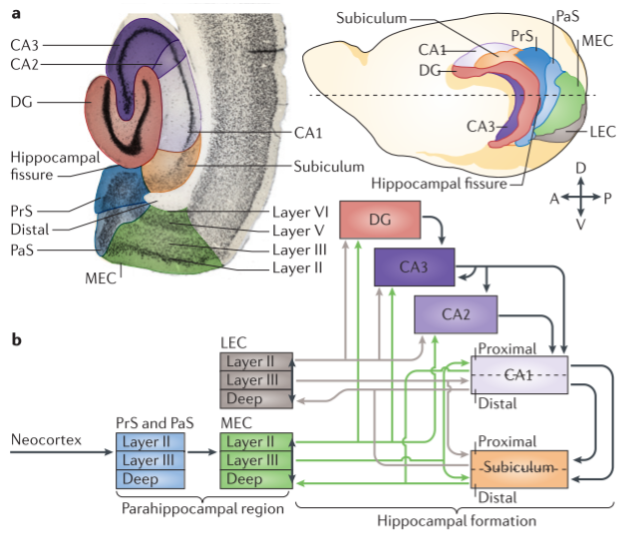
\includegraphics[width=150mm]{figures/F2_HPC_anatomy.png}}
\caption[Hippocampal-entorhinal Anatomy]{
(a) A slice of the right hemisphere of the rat brain (left). The focus is made on hippocampal and entorhinal regions. The same regions are shown located inside the rat brain (right). (b) Schematic of the connections within and between hippocampus and entorhinal cortex (adapted with permission from \cite{Moser2014})
}
\label{fig:F2_HPC_anatomy}
\end{figure}


\subsection{Sequence coding and theta phase precession in hippocampal cells}

As was established in the end of 1960x, hippocampal local field potential (LFP) activity provides oscillations of different modes and frequencies (\cite{Vanderwolf1969}). There are two main regimes - a prominent oscillation in a range between 7 to 12 Hz named Theta oscillation, and other irregular activity with broader spectrum of frequencies, including Gamma periods, Sharp-Wave Ripples (SWRs) and others. In rodents, theta oscillation highly correlates with animal actions and movements - running, jumping, grooming (\cite{OKeefe1993}). Here we focus on the theta regime and the corresponding animal behaviors, as they have an intrinsic connection with hippocampal cells.

Looking more detailed at these hippocampal place cells, an outstanding feature of the place cells behavior is their ability to lock their activity to a certain phase of the theta oscillation, when an animal runs through a place field (Figure 3a). While crossing a place field in one-dimensional or two-dimensional environment, place cell discharges in spiking bursts at progressively earlier phases of the theta rhythm, from spiking at peak of theta oscillation when entering a place field, having the highest firing rate (middle of the place field) on the trough to later spikes when exiting a place field on the ascending phase of theta oscillation (\cite{Jensen1996}, \cite{Skaggs1996}, \cite{Tsodyks1996}, \cite{Dragoi2006}).

This mechanism of spiking bursts within regular time windows is important for linking related path segments using the spike-timing dependent plasticity (\cite{Dan2004}). Importantly, the same mechanism might be useful for successful integration of the coherently incoming feature-extracted information of different modality, like the positional information relative to the spatial boundaries (boundary vector cells) and positional information relative to visual cues or landmarks (visual object vector cells), forming a unique spatial representation. More generally, the same mechanism, when used to integrate non-positional information like odors, sounds, or reward expectations, could be the basis of forming time-invariant memories, or episodes (\cite{Buzsaki2018}).


\begin{figure}
\captionsetup{format=plain}
\makebox[\textwidth]{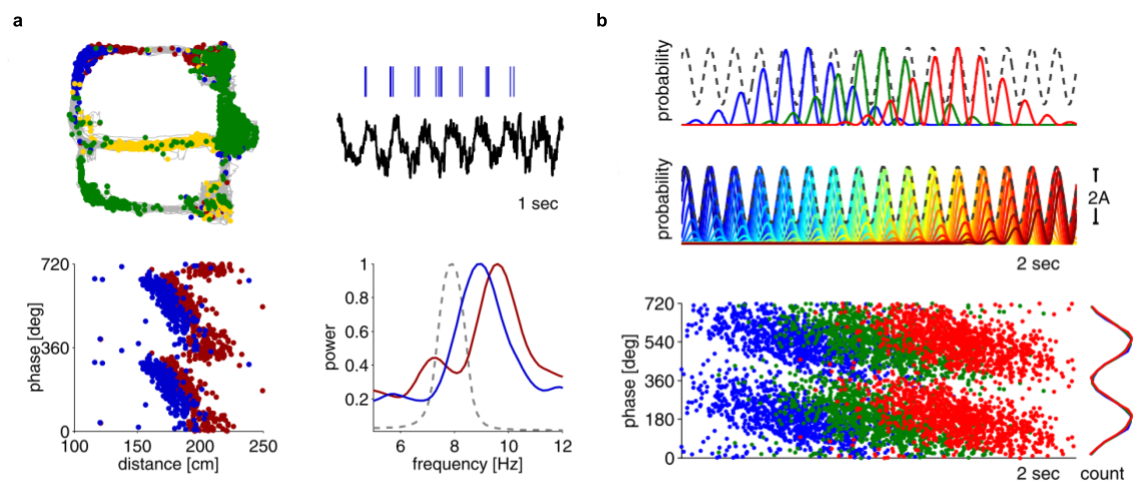
\includegraphics[width=150mm]{figures/F3_phase_precession.png}}
\caption[Theta phase precession]{
(a) A phenomena of the spiking precession of hippocampal neurons relative to the internal LFP theta oscillation. A neuron spiking is chunked by the oscillation and appears earlier in phase as a rat goes through a place field. (b) Sequences of memories and their interference (top), spiking phase relative to the theta oscillation (adapted from \cite{Geisler2010}; permission not required).
}
\label{fig:F3_phase_precession}
\end{figure}



\subsection{Formation of place fields}

Grid, border and head direction cells in the mEC together form one independent representation of space, stable between environments. The reciprocal representation is constructed by hippocampal place cells, that often fully remap between different environments, forming an unique representation of a particular space. These two spatial representations are complementary: one expresses the metric of a space independent of the specific landmarks or action-defined context, another is sensitive to the unique experiences in that space, location of objects or landmarks, building a number of context-dependent orthogonal representations.

The experimental evidence of the increased density of hippocampal place fields near corners and boundaries compared to the center of the environment (\cite{Wiener2737}) leads to a suggestion of a high level of a direct contribution of the border cells to the formation of place fields. Another fact supporting this hypothesis, is that border cells in the mEC are available in the early development - as do place cells when an animal explores an environment on the first day. This leads to an assumption that border cells might have a larger influence on place cells in youth, with the increasing role of grid and other types of mEC cells in adulthood.

Importantly, there is a bidirectional connectivity between hippocampus and entorhinal cortex (see - hippocampal anatomy), the latter receiving feedback from the hippocampus that may be essential for the formation or maintenance of entorhinal spatial maps. This is supported by the experimental evidence that the inactivation of the hippocampal inputs leads to the loss of hexagonal firing pattern of grid cells (\cite{Bonnevie2013}). These facts might be crucial for the explanation of the effects of place cell behavior presented in the results section.

To build experience-dependent representations, place cells need to interact with a variety of entorhinal cell assemblies, carrying distinct types of information. The efficiency and domination of different input types depends on intrinsic properties, like synaptic plasticity, but also on interaction with the environment - animal running speed, behavior, or environmental changes (\cite{Igarashi2014}). It is not yet clear if some of the input types dominate the other, and how place cells recruit synaptic inputs of a certain type to build stable spatial fields. In this work I try to address these questions and to demonstrate that in some particular conditions these inputs of allocentric and idiothetic nature are mixed, and try to further explore the dynamic balance between them.


\subsection{General questions}

The mechanisms that implement spatial navigation in the hippocampal-entorhinal system are not fully described and understood. Among open questions are the mystery behind the formation of the grid patterns, the phenomenon of theta phase precession, the role of gamma oscillations in memory consolidation, how and where the path integration is implemented and many others. Here in this study I focus on the phenomena of place cells in the CA1 region of the hippocampus, especially on the integration of the idiothetic, or precisely boundary-driven information and the visual, landmark driven information into a reliable space representation. The interaction between these allothetic and idiothetic inputs at the level of their postsynaptic influence, especially when they are in conflict, is not yet fully understood. Ultimately, these interactions may reveal, if described in detail, the more general mechanisms of episodic memory formation within the hippocampus which could be extended from navigation to a broad range of behavioral applications, including general action planning and abstract thinking.


%\section{The role of visual landmarks and physical boundaries in spatial navigation}
\section[The role of visual landmarks and physical boundaries in spatial navigation]{The role of visual landmarks and physical boundaries in spatial navigation%
              \sectionmark{The role of visual landmarks and physical boundaries}}
\sectionmark{The role of visual landmarks and physical boundaries}

\label{sec:role_of_landmarks}


\subsection{What is a place?}

A place in physical space can be uniquely defined by a set of reference points and landmarks, similar to it’s representative location on an allocentric map. Place is usually considered invariant of time and independent of the way how a subject gets there. This invariance connects the definition of place to the broader definition of semantic memory - invariant stable description of living things, facts or other knowledge (\cite{Buzsaki2013}). Repeated exploration of the environment allows subjects to revisit the same location multiple times, gradually building its representation from recurrent similar episodes - by linking together different (in time) episodes that share the same set of features, landmarks and relations between them.

High-level feature extraction is necessary to build a coherent representation of space, mainly because early sensory systems predominantly encode very simple stimulus modalities with very localized receptive fields. These would not be enough to build similar episodes sharing the same set of features, in case, for example, an animal reached the same location from opposite sides - and  experienced some different visual flow, experienced a set of new sounds, or made a different number of steps walking from the other boundary. Higher brain areas like hippocampus or cortical areas, involved in both memory and navigation, need to operate with higher order features like boundaries, objects of different shape, visual and olfactory landmarks, in order to be able to combine them as a set of similar combinations of sensory features (episodes) to an invariant representation of a particular location. As was shown in the first section, these operations of high-order feature selectivity might mainly reside in the mEC/LEC, being mostly implemented by boundary, object, and landmark vector cells. As anatomically hippocampus receives its major input from the entorhinal cortices, its role in navigation, shown by place cells, might be to orchestrate these incoming navigational information elements to either build and store a new place memory - a unique constellation of features, representing new location, or to update already existing place memory, if this set of features is similar to the already experienced number of stable objects, shapes and cues at a certain distance.

While external sensory information about distinctive and stable environmental features is necessary to build a stable allocentric map, the internal idiothetic information is required to both support this initial formation, as well as to maintain the constructed representation when the external information is partially or completely not available - for example, in total darkness. Our brains are able to maintain the allocentric position and navigate in space without external inputs, for the price of some error accumulation (\cite{Etienne1988}; \cite{Etienne2004a}). This is an indispensable function of the internal navigation system, essential for successful survival and evolution. The implementation of that feature requires an integration of the information coming from the internal idiothetic system into the circuits, encoding spatial maps. This aspect of establishing, recalling and maintaining the spatial map in absence of sensory inputs are discussed below in this chapter.


\subsection{Landmark and boundary vectors as reference frames to establish spatial map}

Overall, to build a spatial map one needs to define a set of related places (in the brain - place fields) having a certain position within a particular spatial reference frame. A reference frame can be defined as an independent coordinate system, having a definite distance and orientation to one or several reference points. Following this classical definition both environmental boundaries and a set of visually defined landmarks can serve as two independent reference frames, if they don’t change their relational stability between reference points within itself. When it is the case, the aforementioned landmark vector cells and boundary vector cells (\cite{Deshmukh2011}; \cite{Hooydal2019}) can be used to represent two reference frames of different modality in the brain.

While exploring the new environment, these inputs from the boundary vector cells and landmark vector cells (as well as other sensory modalities - olfactory, auditory etc.) are integrated to form coherent stable points, or recurrent episodes, which taken altogether, can be used to form a consistent allocentric representation of the surrounding environment. While moving from one place to another, animal revisits the places, formed of the similar set of environmental features, and reactivates the very similar sensory inputs which, with the help of some pattern completion mechanisms, updates and sharpens the CA1 ensemble representation of a particular physical location - place field in the hippocampal memory system. This movement from one place to another builds a trajectory - a set of connected physical places as an animal path, as well as the set of activated and connected places fields as a virtual path in the brain (\cite{Buzsaki2013}).


\subsection{Mechanisms of path integration to support navigation stability}


To maintain the navigational stability when allocentric cues are removed, the internal navigation system, including place cells, continues to track location using self-motion. Path integration is essentially a computation transforming a change in motion into a change in position. Having a current position estimate, one can derive a new allocentric position by tracking angular movements and distance travelled. Whether this system is based on continuous integration of angular or linear velocities, or on addition of a distance travelled vector to the current estimate - it is based on cues derived from the inputs from the self-motion systems (\cite{Etienne2004a}). These cues include vestibular, proprioceptive cues or motor efference copy (step counting). Additionally, a change in airflow (e.g. sensed by whiskers) or vibration from textures while moving can support speed calculation and resulting translation detection (\cite{Savelli2019}).

How can the path integration system be implemented in the brain circuits? While both distance and angular movement signals coming from grid and head direction cells tend to drift in open spaces without correction by particular cues or landmarks (\cite{Barry2007}), they are still the great candidates to support the path integration system. Boundary cells, or the tactile sensory inputs in the environmental corners, can episodically reset the grid and head direction inputs bringing the path integration system up to date with the environment position and orientation (\cite{Barry2007}; \cite{Cheung2012}). This leads to an assumption that path integration is mainly implemented in the cerebral cortex in a form of an attractor-network (\cite{Knierim2012}; \cite{McNaughton2006}), supported by the fact that the hippocampal upstream regions have all necessary components.

Another reported alternative is that the path integration computations are performed in lower regions, subcortically, reflecting the organization of the head direction system (\cite{Savelli2019}). As thalamic or other subcortical regions already receive vestibular and motor signals, they are able to compute and integrate angular and translational velocity signals, implementing basic path integration. The anatomical structure of the head direction system, for instance, with head direction cells found in anterior dorsal thalamic nucleus (\cite{Taube1995}) is another evidence to support this alternative.


\subsection{Impact on place cells}

Navigation at the level of hippocampal formation with its place cells are the main focus of this study. There is evidence showing that place cells follow visual cues (\cite{Muller1987}; \cite{Deshmukh2013}; \cite{Aronov2014}), suggesting that they receive incoming allocentric information. There is also a large evidence showing that place cells are able to maintain their place preference in case the sensory inputs are removed (\cite{Gothard2001}; \cite{Quirk1990}). In conflicting situations, as was shown in virtual reality (VR) studies (\cite{Gothard2001}; \cite{Haas2019}), cells are able to switch from one to another reference frame in their selective firing, suggesting integration of allothetic and idiothetic inputs. As described in the previous sections of this chapter, initial sensory processing and feature extraction, as well as path integration happens mainly outside the hippocampus. Taken together - how exactly these different pathways are integrated within the hippocampal neural circuits? This question is still not well understood. Below I review a few model studies exploring potential mechanisms of this integration (see modelling section).


\section{Research on interaction of allothetic and idiothetic inputs}
\label{sec:interaction_allo_idio}

One of the first seminal research studies of the effect of the allothetic environmental changes on place cells was done in 1987. Muller and Kubie (\cite{Muller1987}) showed that the rotation of a visual cue card, but not its width or shape, produces rotation of the place fields in a cylindrical arena. Removing the card led to a randomized angular representation of the arena. These recordings demonstrated direct dependence of the place field orientation on the visual information, implicating that cells in the hippocampus are modulated by allothetic visual inputs.

Getting more detailed, several years later, it was shown that objects located near the center of the arena could not control the orientation of the place fields in the environment, but do that with a help of a cue card on the wall (\cite{Cressant1997}). Same objects, placed near the walls enable control over the fields orientation, indicating that involvement of the head direction system, that potentially resets angular orientation relative to the unique objects, located close to the environmental borders.

The question of interaction of allocentric and idiothetic representations got more specificity in later studies by Bures and Zahalka (\cite{Bures1998}), where they experimentally trained animals to avoid foot shocks using either room landmarks or using idiothetically defined area on the floor. The ability of rats to avoid shock locations defined in both reference frames showed credible independence of the allocentric and idiothetic mechanisms, encoding two reference frames. However, a question of how these two systems are intermixed remained unclear.

Gothard and McNaughton proposed that place cells, mainly driven by internal “path integrator” - accumulated internally-driven translational information about a movement in space together with head direction cells - form a preconfigured network of a two-dimensional space. This network is updated by the visually-specific landmark information using associative learning (\cite{Mcnaughton1996}). They performed a series of experiments with rats on the linear track where two separate reference frames were used by a rat to track self position. By gradually moving these reference frames (a reward site and a starting box), they found both cells fired at fixed distances from the origin and cells fired at proximity to the destination. The same neuron was able to shift its spatial preference from being aligned to the origin to an alignment to the destination. They postulate that when mismatches between the visual and the idiothetic information occur, path integration and sensory cues competitively interact to affect place field preference (\cite{Gothard1996}). Their further recordings in light and dark conditions, showing that the box-referenced cells tend to keep their firing preference longer even without light, supported that idea. Ultimately, based on their moving-box-reward experimental data they suggest that interaction between internal dynamics and path integration and external sensory cues happens before both CA1 and CA3 areas, possibly in the entorhinal cortex or subiculum.

However the question of exact mechanism of position computation based on actual or path integrated information remained unclear. A new set of tools including virtual reality was introduced to continue the research of dynamics and circuitry implementing allocentric- and idiothetic- based navigation.


\begin{figure}
\captionsetup{format=plain}
\makebox[\textwidth]{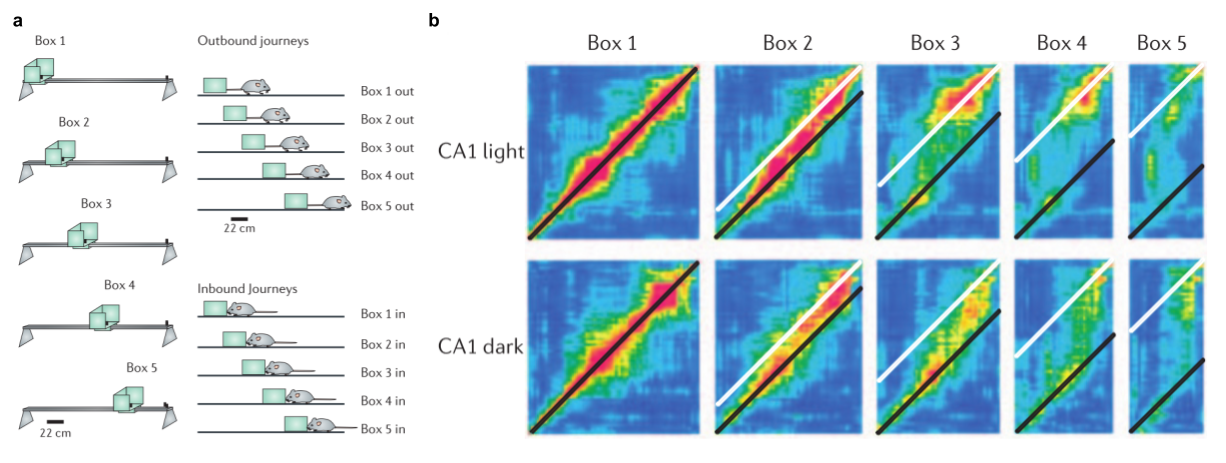
\includegraphics[width=150mm]{figures/F4_moving_box.png}}
\caption[Moving shelter as a reference frame]{
(a) A schematic of the experiment with a moving box. A starting box together with a reward location at the end of the track act as two independent reference frames. By gradually moving the box one can investigate the change of the spatial encoding relative to either of the frames. (b) The resulting place cell firing in light and dark establish gradual shift in encoding position (adapted with permission from \cite{McNaughton2006})
}
\label{fig:F4_moving_box}
\end{figure}


%\section{Optimal combination of environmental cues and path integration during navigation}
\section[Optimal combination of environmental cues and path integration during navigation]{Optimal combination of environmental cues and path integration during navigation%
              \sectionmark{Optimal combination of environmental cues}}
\sectionmark{Optimal combination of environmental cues}
\label{sec:optimal_comb_for_spat_nav}

How algorithmically do the allocentric and idiothetic inputs merge at the level of the hippocampal place cells? When the brain needs to integrate information of different sensory modalities it often uses “optimal” combination - a weighted sum of the inputs with weights proportional to their reliability. This has been established in many behavioral and theoretical studies for humans (\cite{Ernst2002}; \cite{Alais2004}; \cite{Knill2003}; \cite{Hillis2004}) for combinations of different sensory modalities (visual / auditory, visual / haptic, stereo / texture, environmental geometry / path integration etc.). The optimal coding theory is also applicable for spatial navigation. In a series of behavioral studies position estimation based on Bayesian decoding was established and predicted. In particular, optimal cue integration is demonstrated in ants (\cite{Wystrach2015}), rats  (\cite{Shettleworth2005}) or humans (\cite{Zhao2015}; \cite{Chen2017}; \cite{Sjolund2018}). However, while real-world navigation normally implies redundant integration of external, allocentric, cues and internal, idiothetic or path-integration based position estimations, is that combination always optimal?


\begin{figure}
\captionsetup{format=plain}
\makebox[\textwidth]{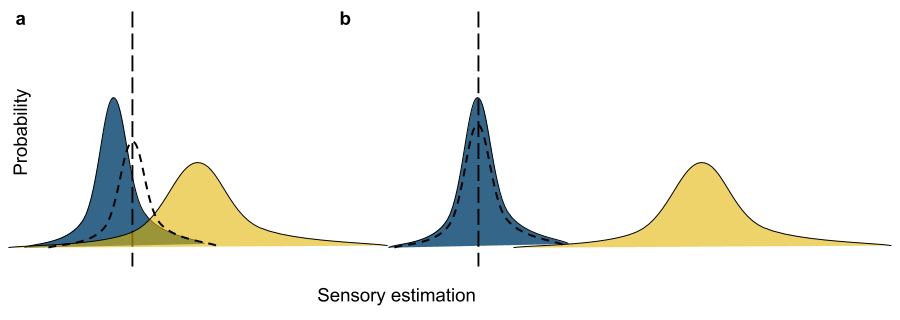
\includegraphics[width=150mm]{figures/F5_larger_smaller_conflicts.png}}
\caption[Sensory conflicts of different size]{
Sensory integration at larger and smaller conflicts. (a) In a situation of a small conflict between estimations it is beneficial to use optimal coding - a weighted combination of the estimation with weights proportional to their reliability (variance). Also named Bayesian decoding, or maximum likelihood estimation (MLE). (b) In a situation of a large conflict between estimations a strategy of abandonment of a less reliable information source will have higher chances to end with a better precision.
}
\label{fig:F5_larger_smaller_conflicts}
\end{figure}


Intuitively, when the conflict between two given estimations is small, weighted integration and resulting averaging makes sense. Especially if performed in an optimal, Bayesian way, it allows for a maximization of the precision of the resulting estimate, attributing a conflict to a sensory noise (Figure 5a). On the other hand, situations of a large conflict might be caused by misidentification of an object identity, incorrect memory retrieval or in general - failure in estimation based on a particular sensory source. In that case Bayesian integration might lead to large errors relative to both information sources, while full abandonment of one, ideally less reliable, source of estimate might be a logical choice (Figure 5b). This abandonment of one source, or cue, in favor of the other has been demonstrated in animal and human navigation studies. For instance, when humans were presented with a large > 115 degrees conflict between landmark and path integration cues they prefered path integration (\cite{ZHAO201596}). Rats in large spatial conflicts also prefer to rely on path integration in favor of a single landmark (\cite{Shettleworth2005}).

While the ability of a brain to implement optimal coding is well known, however it has not been thoroughly explored at the physiological level. Different potential schemes, including gain field theory, convolutional encoding, doubly distributional population coding were introduced (see review in \cite{Pouget2003}), however it is still not clear which scheme is used by the neurons or whether neurons actually encode continuous distributions at the population level. In this work, we address this question and make an attempt to show on the cellular level how these mechanisms of estimation integration at small conflicts and estimation abandonment at large conflicts could be implemented by a population of hippocampal neurons. We hypothesize that attractor dynamics in the hippocampal circuits might implement nearly-optimal coding for spatial and potentially non-spatial estimations, predicted earlier in other sensory systems (\cite{Jeffery2016}) and how the abandonment of less reliable estimation could be implemented at the level of a single neuron.


\section{Modelling multisensory integration at the level of place cells}
\label{sec:modelling}

“…Each place cell receives two different inputs, one conveying information about a large number of environmental stimuli or events, and the other from a navigational system which calculates where an animal is in an environment independently of the stimuli impinging on it at that moment. The input from the navigational system gates the environmental input, allowing only those stimuli occurring when the animal is in a particular place to excite a particular cell…” - an original sentence by O’Keefe led to a general proposal that the place cells might integrate idiothetic information coming from the different cell groups from the entorhinal cortex with some other sensory information.

Initially, a discovery of grid cells led to a model proposed by Solstad and Einevoll, which assumed formation of place cells via linear summation of weighted inputs from the grid cells (\cite{Solstad2006}). It was suggested that irregularly spaced place fields can appear as a result of summing inputs from entorhinal cells with different spacing and orientation, and relatively similar grid phases. However, this model was free from complex network interactions and required having place cells integrating grid cell inputs with overlapping vertices. This issue was fixed later by demonstrating that adding fast hebbian plasticity may result in the careful selection of appropriate inputs, without the need for specific network wiring (\cite{Savelli2010}).

The discovery of border cells and boundary vector cells led to another approach, assuming that environmental boundaries can serve as determinants of the hippocampal place fields. The boundary vector cell model (\cite{Barry2006}) describes place fields emerging from a combination of cells active at a certain direction and orientation relative to the environmental boundaries.

However, both of these approaches were focused on feed-forward type of information transfer, uni-directional communication between cortex and hippocampus. Recently, a novel approach connecting feed-forward information flow from the entorhinal layers to the hippocampus with feedback flow to the entorhinal areas, was proposed (\cite{Li2020}). It is a model that assumes continuous interaction between grid and place cells, with plasticity mechanisms enabling balance in control over place definition between vision and self-motion, allocentric and idiothetic inputs. In this model, self-motion is represented by multiple layers of grid cells that integrate angular and translational movement velocities (see grid cells). Visual input is modelled using a retina-like grid with Gabor filters, applied to the incoming stream of camera images. It is also assumed that it gets input from the head direction system such that the resulting visual information in particular location is independent from head orientation, similar to the non-grid cell in the LEC (see object-vector cells). Competitive organization of the network outputs establishes two different populations of place-selective cells - purely self-motion (or boundary) driven (motion place cells - MPCs), and purely visually driven (visual place cells - VPCs). These cells are assumed to be present in the CA3 regions of the hippocampus and together provide informative inputs to CA1 place cells. Having hebbian plasticity mechanisms and feedback connections back to the self-motion grid cells (MPCs), these latter CA1 cell are classified into 3 major groups - visually driven, self-motion or boundary driven and multisensory cells, that combine both of the allothetic and idiothetic inputs. These simulation results are very similar to the previously reported results (\cite{Haas2019}), as well as they highly correlate to the new electrophysiological data from the current study. Here I found very similar groups of neurons, having similar spatial firing properties (see Results). However, the disadvantage of the model is that it does not account for border-defined inputs which, as we also find in the neural data, might play an important role in correcting self-motion vectors and modulating the dynamics of the network as a whole.

Ultimately, considering models of the underlying neural dynamics, the current work is attempting to provide additional evidence for the modern loop-based approach to describe hippocampal-entorhinal networks implementing principles of spatial navigation. Based on the collected data, we hypothesize that hippocampal neurons implement a weighted combination of position estimation based on allocentric and idiothetic inputs in a nearly-optimal fashion. We show that the resulting position estimation influences self-motion based place representation, possibly via backprojections from the hippocampus to the entorhinal cortex. Overall this makes a step towards bringing evidence based on the neurophysiological data for the proposed model in situations, when place definitions are conflicting.


\section{Aim of the thesis}
\label{sec:aim_of_thesis}

For many years hippocampus has been identified as a brain structure, critical for spatial learning and navigation. The spatial domain extends beyond the traditional navigation in physical spaces - to many abstract spaces humans need to operate daily, not only to be partially efficient, but also to be successful in survival. Hippocampus, having specially tuned neurons - place fields - that rely on external sensory inputs and self-motion cues, mainly coming from the cortical areas, is able to implement high-level context-dependent representation of the environment. However it is still not known how exactly these different information flows interact to build a consistent and stable map of connected place fields.

Existing studies suggest that both proprioceptive and idiothetic types of information are continuously integrated to update the self-position (e.g. implementing “path integration”) while other stable sensory cues provide references to periodically update the allocentric position of self and correct it for the collected integration-related errors. It was shown that both allocentric and idiothetic types of information influence positional cell firing, however in most of the studies these inputs were firmly coupled. The use of virtual reality setups (\cite{Thurley2016}) made it possible to separate the influence of vision and proprioception for the price of not keeping natural conditions - the animal is usually head- or body-fixed (\cite{Holscher2005}; \cite{RavassardA.2013}; \cite{Jayakumar2018}), which introduces vestibular motor- and visual- conflicts, providing a bias for space encoding. Here we use the novel CAVE Virtual Reality system for freely-moving rodents (\cite{DelGrosso2018}) that allows to investigate the effect of visual- and positional- (vestibular) manipulation on the hippocampal space code while keeping natural behaving conditions.

Particularly, the current research is aimed at studying the impact of visual and vestibular (passive translation) manipulations on the hippocampal code using this novel freely-moving ratCAVE system. With the ability to manipulate the projected virtual environment and to unidirectionally move the physical arena depending on animal’s position, the following questions are addressed:

\begin{itemize}
  \item how would the stable visually-defined spatial reference frame impact the hippocampal place code when put in conflict with the moving space reference frame, defined by the physical boundaries
  \item would the passive physical move in space, locked to the physical boundaries and supported with vestibular inputs, differently impact the place code in contrast to the opposite situation when the move of the reference frame is just visual and not supported by the vestibular inputs - addressing the question of the role of vestibular information in coding the preference to one or another reference frame
	\item whether an instant mismatch between the visual and proprioceptive inputs (gain) would distort the hippocampal place map and at which threshold
	\item what types of the hippocampal place cells could be separated by their sensory and / or feedback inputs (visual, self-motion or boundary-driven or their combinations) and how strong is the path integration component
	\item whether a single instant conflict between information coming from the internal path integration system and the visual information can influence the current place code or lead to any remapping
\end{itemize}

In summary, we focus on the dynamic representation of space when the visual-cue-defined and physical-boundary-defined reference frames are in conflict. We confirm the dominance of one reference frame on the other on the level of place fields, when the information about one reference frame is absent (\cite{Gothard2001}). We show that the hippocampal cells form distinct categories by their input preference - surprisingly, not only that they are being driven either by visual / allocentric information or by the distance to the physical boundaries and path integration, but also by a specific combination of both. I found a large category of units integrating inputs from both allocentric and idiothetic pathways that are able to represent an average location between two reference frames, when they are in conflict. The use of virtual reality allowed me to demonstrate that these units become only path integrator driven when they lose their visual inputs. Based on the recorded information about these single cell theta phase-modulation, I propose a model how these units can integrate allocentric and idiothetic inputs to form this independent category of place representation.

Ultimately, the aim of the current work is to try to provide more support in linking the view over the hippocampus from the other side - to consider it not only as a spatial machine, but as a common generator of sequences of episodic memories (\cite{Buzsaki2013}), having place cells as examples of a particular recurrent episode - an integrated internal and external feature-processed sensory information at a particular moment of time, shaped by brain theta rhythms.


\chapter{Experimental Design and Procedures}
\label{ch:design}

\section{Using Virtual Reality to study navigation}
\label{sec:using_vr_navigation}


An efficient strategy that advances understanding of the complex spatial representation system is based on perturbation of one of its components. Experimental approaches using Virtual Reality systems (VR) allow to selectively perturb and manipulate visual cues. In recent years these systems have been widely used to study navigation (\cite{Holscher2005}; \cite{RavassardA.2013}; \cite{Aronov2014}; \cite{Thurley2016}).

The development of virtual reality (VR) systems for rodents (\cite{Holscher2005}) enabled scientists to manipulate environmentals properties, such as visual cues and landmarks in a fast and accurate way. It was shown that, despite the absence of the normal vestibular motion signals or tactile border inputs, animals are able to navigate in virtual coordinates, as well as their similar spatial neuronal metrics like place cells in the hippocampus are preserved. Chen and O’Keefe demonstrated that in VR, similar to the real environment, movement and visual information are combined nonlinearly in the place cell activity; the influence of one (visual) or another (proprioceptive) component varied significantly across cell population (\cite{Chen2013}). However, while being a good tool for sensory manipulation, body-fixed VR systems cannot fully model navigational processes in the brain - they do not only reduce theta frequency and speed dependence, but also reduce the number of active place cells and affect their directionality (\cite{RavassardA.2013}).

Although only simulating real environments and spatial navigation, VR systems opened a large door to the investigation of the neural behaviors when sensory inputs of different types are in an instant conflict. By introducing a gain-like difference between the speed of the visual projection and self-motion, one could establish a distinct population of neurons that either were locked to the salient visual cues or were strongly influenced by animal’s locomotion (\cite{Jayakumar2018}, \cite{Haas2019}). A set of experiments with continuous conflict between path integration and visual landmarks resulted in demonstrating stable and prolonged recalibration of the path integrator by the external information. This evidence supports the idea that visual cues do not only correct accumulated path integration errors, but can quickly reset the sense of position and update appropriate path integrator computation (\cite{Jayakumar2018}). The very recent work exploring hippocampal CA1 - CA3 regions shows highly context-dependent spatial coding in these regions (\cite{Zhao2020}), suggesting a high level of pre-processing of environmental features before they reach hippocampal formation.

Looking outside the hippocampus to the entorhinal cortex, gain experiments in VR revealed that border cells are mainly locked to the visual landmarks, while grid cells are modulated by both locomotion and optic flow. In the same set of experiments it was shown that the visual optic flow becomes more influential if it’s faster than expected (\cite{Campbell2018}). The recent mEC recordings show a new class of visual cue cells - neurons exhibiting firing fields near visual cues, consistently across different environments (\cite{Kinkhabwala2020}). This is another evidence that the entorhinal cortex contains both representation of landmarks and physical boundaries, - enough information to perform proper path integration.

However, while enabling outstanding opportunities for visual sensory input manipulations, conventional VR systems require animals to be body- or head-fixed. This poses a series of difficulties with animal training, imposing a different animal state (e.g. fear, aversion), as well as keeping some of the sensory information sources (e.g. vestibular, or olfactory) in a non-natural condition. These head- or body behavioral restrictions distort partially the vestibular and proprioceptive inputs and may lead to differential effects on place cell maps (\cite{Stackman2002}). Altogether this significantly impacts the navigation - both behavior and neural code.

To address these issues a freely-moving VR system ratCAVE was built (\cite{DelGrosso2018}). In contrast to conventional VR systems (\cite{Thurley2016}), ratCAVE allows for a natural animal movement and exploration in a rectangular arena, while retaining the possibility to manipulate distal and proximal (virtual) visual cues to influence animal navigation. It avoids vestibular motor and vestibular visual sensory conflict during locomotion, while constantly updating the surrounding virtual environment via the subject’s own freely-moving head movements, supporting natural perception and behavior. In addition, the ratCAVE setup (see Methods) enables to physically move the arena, partially distorting vestibular and proprioceptive inputs and changing the allocentric position of the animal.


\section{Experimental protocols}
\label{sec:protocols}

To study the role of different components of the allothetic and idiothetic systems on the hippocampal place code we introduce a conflict between different sensory inputs using Virtual Reality. We manipulate visual (virtual, projected) relative to the physical (defined by arena boundaries, tactile) reference frames as a key instrument to implement this mismatch while recording hippocampal CA1 neurons. By comparing the original condition, where both visual and boundary-defined reference frames are aligned, with the non-matching condition, where these frames are in conflict, one could study the dependency of the place cell activity on the navigation relative to one or another frame, as well as how intrinsic path integration would influence single unit activity.

\begin{figure}
\captionsetup{format=plain}
\makebox[\textwidth]{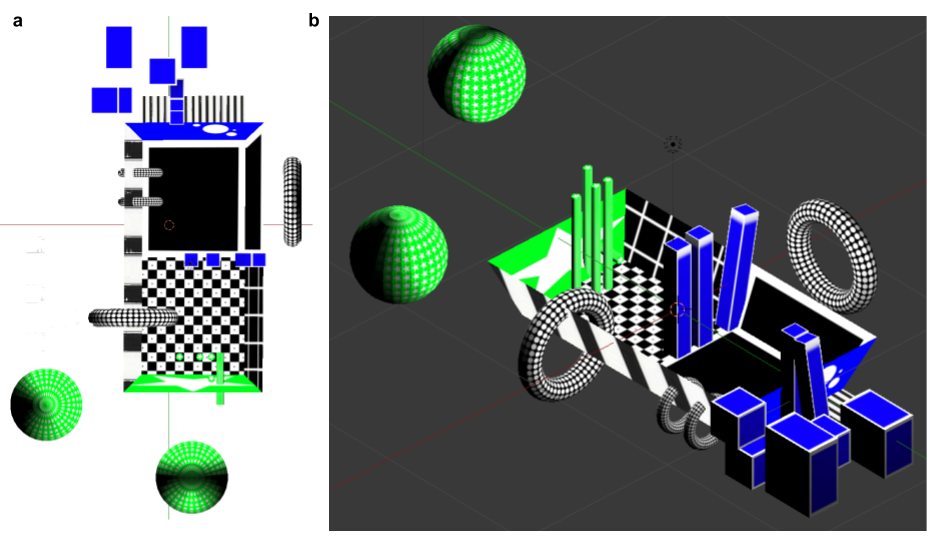
\includegraphics[width=150mm]{figures/F6_virtual_scene.png}}
\caption[Design of the Virtual environment]{
Model of the virtual environment for the ratCAVE Virtual Reality setup. (a) Top view of the Virtual environment for vSHIFT and vGAIN experiments (b) Same virtual environment viewed from the Blender modelling software to better see virtual objects and separation in three visually-distinct compartments.
}
\label{fig:F6_virtual_scene}
\end{figure}

The virtual environment consisted of the proximal and distal elements. Distal landmarks were unreachable, they consisted of two green spheres and several blue bricks located at some distance around the arena. The proximal landmarks are represented by landmarks on the arena walls - black and white stripes, black and white plaid, a grey star on a green background, together with distinct visual patterns on the floor - checkerboard pattern, black square pattern, stripes pattern, and virtual objects inside the arena - torus of several sizes, blue and green tall vertical bars. These objects and patterns supported the split of the virtual environment in three distinct “compartments”, which were chosen specifically to induce maximum visual influence on the animal visual perception system and engage more neurons in coding the visual reference frame (see Figure 6). For example, the “stripes” compartment in the vSHIFT -physical experiment is hidden in the original position of the arena, but is available to the animal in the shifted position. At the same time salient green bars on the other end are not reachable, which overall might induce visually-driven cells to more prominently react on the change.

For all shift and gain experiments animals were kept on the light food diet (about 90\% of ad libitum weight); animals were randomly foraging for food pellets inside the ratCAVE arena (see methods). Experimental time and movement protocols are described in detail in the following sections.


\section{Introducing mismatch between stable reference frames}
\label{sec:mismath_frames}

The aim of this experimental series is to identify the distribution of a subset of external sensory inputs (visual, tactile or boundary-defined) to the hippocampal place cells and the interaction of these inputs with the internal self-motion (proprioceptive, vestibular) signals, crucial for path integration. By probing whether the place fields would follow the 3D virtual visual reference frame or the physical boundary-defined arena frame one could split the influence of visual versus tactile (corner- or boundary- related) stimulus and determine how much they are influenced by path integration.

\begin{figure}
\captionsetup{format=plain}
\makebox[\textwidth]{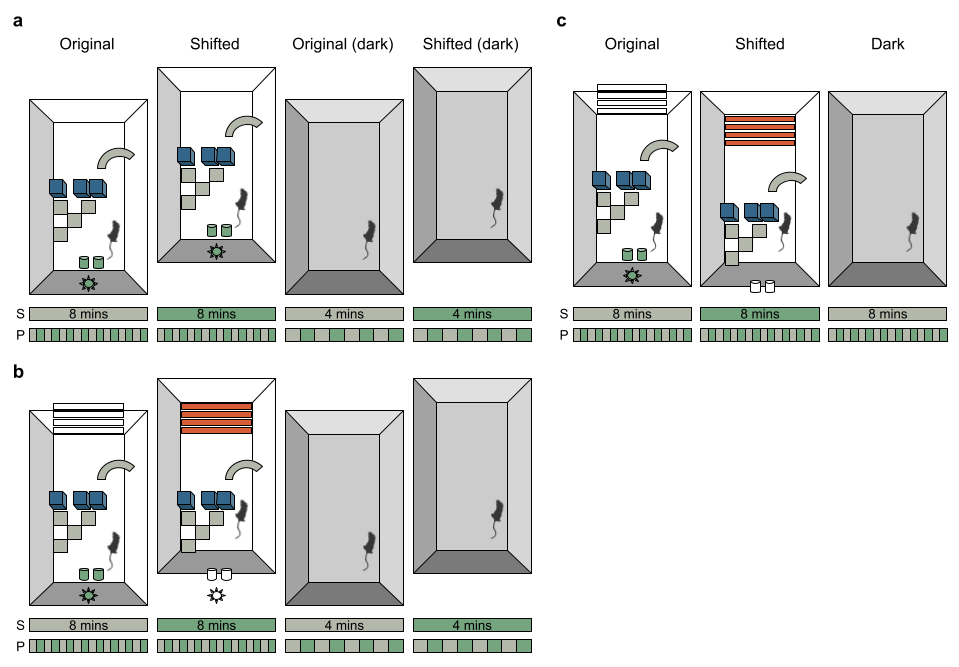
\includegraphics[width=150mm]{figures/F7_vSHIFT.png}}
\caption[vSHIFT experiment]{
Schematic of the concept of the vSHIFT experiment. For all plots: the green/gray bars on the bottom determine the protocol of the arena movement between original and shifted positions. S (single) - a single move, P (periodic) - translation every 30s. (a) vSHIFT - coherent. ratCAVE arena is translated together with the projected virtual objects and visual cues  back and forth along one axis, while the animal is randomly foraging inside. (b) vSHIFT-physical. The arena is periodically translated back and forth while the visual projection (virtual environment) is kept stable in room coordinates. (c) During vSHIFT-visual the arena is kept stable while the visual projection is translated further and back at the same protocol as in (b).
}
\label{fig:F7_vSHIFT}
\end{figure}


\subsection{vSHIFT-coherent - no conflict between reference frames}

To provide an evidence, that the external room cues (e.g. a projector and a mirror) do not play a role in formation of the spatial map, we designed an experiment where the both the arena and the visual scene were moving congruently together in the same time and spatial order as in the previous experiments. As these cues are subtle and hardly seen it is expected that they are ignored by the sensory inputs and do not influence spatial information in the hippocampus as well as the mechanisms of path integration. More precisely, it is expected that none of the units are able to fixate their spatial firing to the room reference frame, and all place fields would move together with the arena and the aligned visual scene. In addition to the experimental evidence of reference frame preference, the resulting distribution of the shift of the place fields could provide statistical metrics (e.g. standard deviation) for these particular conditions (arena length, animal size and behavior), useful for future analysis of other experimental conditions.

In this experiment both the arena and the visual projection were physically moved every 30 seconds in a longitudinal direction for 0.3 meters forth (shifted position, B) and back (original position, A), using the linear actuators located below the arena, like in the physical shift experiment. This action kept visual and border-defined reference frames aligned, while passively moving an animal in allocentric room coordinates (Figure 7a).


\subsection{vSHIFT-physical - conflict between vision and path integration}

In this experiment, a stable visual projection of the 3D virtual environment, containing proximal (virtual bars, torus and pillars) and distal (spheres) landmarks, was projected on the walls of the physical ratCAVE arena. This projection was stable in room coordinates for the whole experiment. To implement a shift, the arena was physically moved once or every 30 seconds in a longitudinal direction for 0.3 meters forth (shifted position, B) and back (original position, A), using the linear actuators located below the arena. The acceleration of the move was above the detection of the vestibular system, supporting the animal feeling of "being moved". As the projection was stable in room coordinates, it appeared to “shift” inside (relative to) the arena because of the arena move. This introduced a shift between the spatial reference frame, defined by the physical arena boundaries, relative to the visual virtually-defined VR reference frame (see Figure 7b). Neuronal activity was recorded during the whole session, and later only the times when the arena was stationary were analysed. For condition analysis, all periods when arena was in either original (A) or shifted (B) position were integrated to form two separate conditions A and B. For all animals, the session duration was ranging from 12 to 16 minutes, resulting in approx. 6 to 8 minutes of recording in condition A (12-16 arena moves) and 6 to 8 minutes in condition B (12-16 arena moves back).

For some sessions a 8 minutes period of an animal foraging in total darkness was recorded. These result in approx. 4 minutes of recording of the same neuronal units in position A and 4 mins in position B in darkness.

The shift of the arena to position (B) allowed an animal to enter a new virtual area, not available previously in original position (A). This area is marked by horizontal stripes (see Figure 7b, orange). Simultaneously, a virtual area at the end of the virtual scene (with green pillars), was no longer available in position (B) as the physical arena wall prevented an animal from going there. The salient visual landmarks (stripes, pillars) were specifically designed to be present in these areas to engage more place cells to change their activity in two shift conditions.

It is expected that this experiment allows to classify cells by their visual and/or self-motion or boundary-defined selectivity, thus suggesting their possible upstream input types. By studying the way the two different reference frames are represented by place fields may indicate the way the integration of these pathways is processed in the CA1 pyramidal layer.


\subsection{vSHIFT-visual - alternative way for a conflicting condition}

To probe whether the passive physical movement in space, supported by vestibular signals, is crucial for physical or visual reference frame encoding, it was asked if the shift of the visual scene alone could induce the shift in the encoding of the spatial map. Opposite to the previous physical shift experiment, here the visual projection, containing all distal and proximal virtual landmarks, was moved relative to the stable arena. In original position, the projected virtual scene matched the arena walls similar to the previous experiment, condition A. To introduce a shift, the visual projection was moved every 30 seconds in a longitudinal direction for 0.3 meters forth and back with the same timing, as it would take the physical arena to move. As the physical arena was stationary during the whole experiment, this move introduced a shift between the spatial reference frame, defined by the stationary physical arena boundaries, relative to the changing visual reference frame, with the exception that the animal was not physically moved in room coordinates and the vestibular input pathways were not stimulated (see Figure 7c).

This experimental condition is similar to the physical shift condition but without the translation of the animal and the arena in space. As the physical move engages vestibular inputs, this might influence the encoding of one or another reference frame in the hippocampus and might be interesting for a separate research.


\section{Introducing mismatch between vision and proprioception}
\label{sec:mismatch_gain}

The invention of different types of virtual reality setups for rodents (\cite{Thurley2016}) allowed to study the activity of the hippocampal cells when visual flow and self-motion are in continuous conflict. Tracking the position of the animal at high frequency enabled instant manipulation of the incoming visual flow inducing permanent gain mismatch between the actual translation (e.g. a real number of steps travelled) and the translation in the virtual space (e.g. the distance in virtual coordinates). Many studies claimed the ability of the hippocampal place cells to encode visual landmarks (\cite{Chen2013}; \cite{Aronov2014}; \cite{Jayakumar2018}) as well as the distance travelled (\cite{Haas2019}) in both gain and no gain conditions. However, as mentioned previously (see - using virtual reality to study navigation) in the head- or body-fixed VR systems some signals from the vestibular system (e.g. otoliths) are not present, while is has been shown that the vestibular system has a significant impact on the formation and stability of the place cells in general (\cite{Stackman2002}). Additionally, the ball-VR setups do not provide any real boundaries, making complex to bind position encoding based on self-motion to the environmental geometry. This series of VR experiments in freely-moving condition targeted to investigate effects on the hippocampal CA1 activity when there is either an instant or spontaneously induced mismatch between visual landmark-defined information and the self-motion, path integration defined information.


\subsection{vGAIN - shift via introducing a gain mismatch between visual flow and proprioception}

Another way of studying the preference for visual versus boundary-defined reference frames for spatial navigation is to introduce a gain mismatch between actual animal movement and the visual flow. Using the VR system, this can be implemented as essentially letting the animal move for a certain distance while moving the visual scene for the same distance multiplied by a coefficient.

To keep all the series of experiments compliant and comparable, we introduced the linear longitudinal gain of the visual flow of 1.2 and 1.5 between the virtual scene and the animal physical translation in a series of 3 stages: original no gain condition, gain condition (when an animal can access extended environment in VR coordinates) and again the no gain condition, when the virtual scene is shifted relative to the arena reference frame (see Figure 8a). Intuitively this experiment is similar to the physical or visual shift experiments (above), with the difference that the shift is performed with the transition via the gain period, when there is a mismatch between the animal longitudinal translation in physical and virtual coordinates.

Each period consisted of 6 minutes recording in every condition with 1 minute between periods, when the gain was linearly increased or decreased. This smooth increase of the gain was required to avoid instant change of the animal position in virtual coordinates and, as a consequence, potential remapping. For some sessions the dark period of 6 minutes was recorded. Recording cell activity in darkness can help in analysis and definition of cells, dependent on visual inputs and their firing behavior after the visual input is cut.

\begin{figure}
\captionsetup{format=plain}
\makebox[\textwidth]{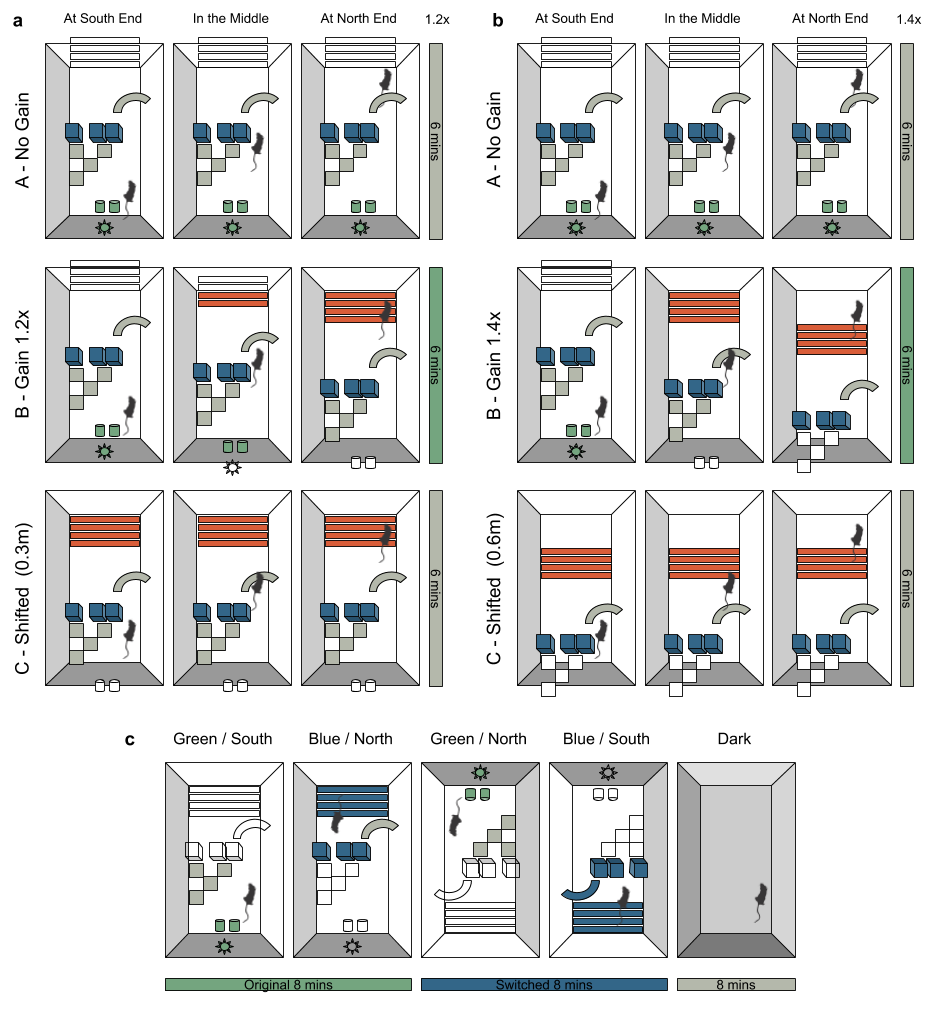
\includegraphics[width=150mm]{figures/F8_vGAIN.png}}
\caption[vGAIN experiment]{
(a) Schematic representation of the vGAIN experiment. Experimental session has 4 periods of original position condition when the animal learns the environment (top row), followed by a gain condition with the extended visual environment fit inside the same physical environment (middle row), and a shifted position condition, where there is no gain but the visual projection is shifted 0.3m relative to the original condition (bottom row). Some sessions followed by a navigation dark (4th period, not shown). Note the visuo-idiothetic spatial conflict between original (A) and gain (B) conditions depends on the position inside the arena (middle row, the conflict is largest at the north of the arena, while there is no conflict on the south of the arena). (b) The same protocol for the vGAIN 1.4x. The difference is the amount of instant (middle row) and resulting (bottom row) conflict ranging from 0 to 0.6m. (c) Schematic representation of the vTELEPORT experiment. Animals learn the environment where the green room is located on the south, and the blue room on the north. Note the projection for only one room where the animal currently is, is active at the same time (left two columns). After an exploration period, green and blue rooms are switched (green room goes north) bringing the conflict between visual cues and path integrator (middle columns). The main conditions are followed by a period of foraging in the dark.
}
\label{fig:F8_vGAIN}
\end{figure}


\subsection{Teleport experiment}

Place cells build spatial maps based on coherent sensory and self-motion-based representations. According to the accumulating evidence (\cite{Gothard1996}, \cite{Samsonovich1997}, \cite{Derdikman2009}) these maps are discrete for distinct environments, associated with unique experiences. Inconsistency between the actual sensory inputs and the recent position history, defined by self-motion and path integration, may introduce a specific type of remapping of the active place representation, referring to one or another discrete spatial map or having a mixture of components (\cite{Jezek2011}).

To study these effects on the level of hippocampal place cells, I designed a virtual teleport experiment. Using the freely-moving virtual reality setup, I designed an environment containing two visually distinct rooms of the same size, that fit the physical VR arena (rooms A and B). While an animal explores room A, the room B was not rendered, so only one room was visually available at a time. Crossing the midline of the arena allowed an animal to move between the rooms. Each room had a hidden circular spot, defined by the proximal visual cues, where an animal could trigger a reward if it stayed within the spot for more than 2 seconds. The rewards were continuously altered between rooms A and B to enforce an animal to navigate between rooms. After the initial learning of the environment for 8 minutes, rooms were switched at the earliest midline crossing, such that it appeared to the animal that it was entering the same room. The switch of the rooms was the central point to investigate whether the mismatch between the previous trajectory (path integration) and a newly imposed visual sensory cues would result in a map substitution or any other type of change in the corresponding place field representation (see Figure 8c).

Due to the time limitations only behavior, but not physiology was recorded with two animals. Behavior recordings demonstrate the ability of animals to learn the reward locations before the switch, as well as quick adaptation to the new orientation of the virtual environment after the room switch (see Figure 8c). This shows the significance of the visual-based virtual representation in original and switched versions and its very probable impact on the spatial map in the brain. However how this teleportation affects the place field maps remains to be investigated.


%\section{Comparison of hippocampal spatial activity between ball- and freely-moving VR systems}
\section[Comparison of ball- and freely-moving VR]{Comparison of hippocampal spatial activity between ball- and freely-moving VR systems%
              \sectionmark{Comparison of ball- and freely-moving VR}}
\sectionmark{Comparison of ball- and freely-moving VR}
\label{sec:comparison_ball_vr}

Previous research on the influence of sensory conditions on the hippocampal place code shows that inactivation of the vestibular system, which severely disrupts the head-direction system, was able to disrupt spatial maps in the hippocampus (\cite{Stackman2002}). While conventional ball-virtual reality systems impose behavioral restrictions such as head- or body fixation they distort parts of the vestibular and proprioceptive inputs, which may result in deformation effects on place cell maps. Understanding the levels of these distortions might be crucial to understand the contribution of self-motion cues to the expression of place fields. The presence of both types of virtual reality setups (ball-VR and ratCAVE VR, see methods and also \cite{Thurley2014}) on-site provided an opportunity to design experiments that compare neuronal activity involved in navigation between the setups, even in the same animal. By recording simple random foraging in the same virtual environment in body-fixed and freely-moving conditions, one could compare neuronal activation patterns, detect differences in place field firing and ultimately better understand the contribution of the vestibular inputs and physical boundaries on the hippocampal place map.

\begin{figure}
\captionsetup{format=plain}
\makebox[\textwidth]{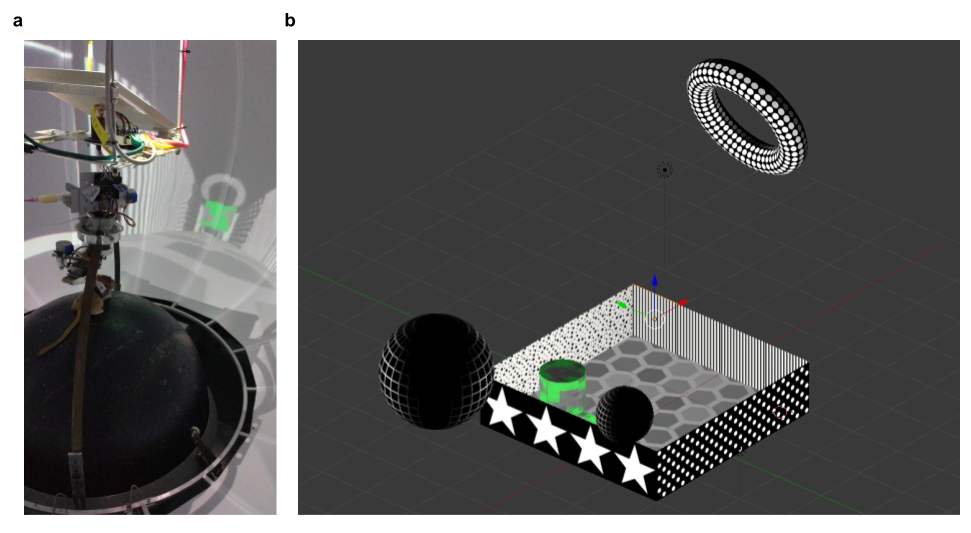
\includegraphics[width=150mm]{figures/F9_ball_VR.png}}
\caption[Ball virtual reality setup]{
Body-fixed virtual reality system. (a) A photo providing an overview of the setup with an animal inside. Animal is held in a harness fixed to the commutator that allows for a 360 degrees rotation. Running on a ball treadmill implements movement in the virtual environment, projected on the screen around the animal. (b) Schematic of the 2D virtual environment used in the beacon navigation task.
}
\label{fig:F9_ball_VR}
\end{figure}

To implement this experiment, I adopted the rendering engine and wrote experimental control software that enables the rendering of the same virtual environment in both VR setups (see methods). I designed a simple 2D environment and a beacon foraging task where gerbils need to navigate to a green beacon, which was changing its position every trial, to get a reward (20mg sucrose pellets in the ratCAVE setup, a 0.1ml dose of sweet milk in the ball setup).

While a freely-moving situation does not require any specific pre-conditioning, ball-virtual reality requires extensive handling and animal adaptation to being restricted by a harness. In gerbils, this restriction does not always lead to a successful animal adaptation and, empirically, depends on animal age, personal character and status in the cohort. As a result, many animals do not feel comfortable in the harness or even build aversion to both harness and setup. Practically this results in either animal freezing while being in the setup on the styrofoam ball, or a periodic running in a single direction, supposedly ignoring the visual projection, with an appearance aimed at escaping. Overall, such animal behavior even after extensive training and adaptation (4-5 weeks) does not always allow for navigation in a 360 virtual 2D environment. Actual training results show on average one out of four animals capable of adapting to the harness and setup, learning the 360 rotation, reward system and 2D navigation for a salient green beacon (not shown in this work). This imposes restrictions on the timing for the surgery: first - one has to train animals to select the right candidate, and second - it increases the risk of an overall wasted time, in case the surgery or recovery does not go well. Ultimately there was a decision to freeze this type of experiment until there is a better and more stable solution for animal training and harness adaptation.


\chapter{Materials and Methods}
\label{ch:methods}

\section{Electrophysiology}
\label{sec:ephys}

\subsection{Subjects}

All experiments were conducted with Mongolian gerbils (Meriones unguiculatus). Gerbils were selected as an experimental animal for a number of reasons. First, gerbils were shown to have a good visual acuity (~ 1.75 cycles/deg grating acuity at 70 cd/m2; \cite{Baker1983}) and visual alertness (\cite{Ingle1981}). Second, gerbils are more active in the light part of the day cycle (\cite{Naumov1975}), suitable for experimental recordings. Finally, gerbils show better exploration of novel contexts and less dependency on moving along the boundaries (thigmotaxis) (\cite{STUERMER2003249}), which is highly important to reach high levels of arena occupancy across all experimental conditions.

In total, 9 wild-type animals from the local breeding facility were used. Among those, all 9 were used in the shift experiment, and 4 were recorded in the gain experiments, so some animals took part in both experimental paradigms. After the implantation of microelectrodes, animals were housed individually with a maintenance of the 12 hours light/dark cycle. A few days after the surgery and before the start of the experiments animals had ad libitum access to food and water. During the recordings, animals were kept on a food diet to maintain 90-95\% of their original ad libitum weight to increase the interest in random foraging for food pellets during the recording. All experiments were approved according to national and European guidelines on animal welfare (Reg. von Oberbayern, license number AZ 55.2-1-54-2532-70-2016).


\section{Implant design}
\label{sec:implant_design}

In the beginning, we used 4- or 8-tetrode Axona microdrives (Axona Ltd., U.K. http://www.axona.com/) to record from the dorsal CA1 region of the hippocampus. Later in the project, aimed at increasing the density of the recording sites in the brain area of interest as well as to have a possibility to reuse recording devices we chose the 32- and 64-channel Buzsaki H64 silicon probes as candidates for electrophysiological recordings. In order to support implantation, maintenance and successful recovery of the probe after the end of the experiment, a set of custom components was designed. These include the microdrive, the base plate, the protecting box and a set of components supporting the implantation procedure.

\subsection{Microdrive}

The industrial microdrives (e.g. nano-Drives from Cambridge NeuroTech) are usually very expensive and do not allow reusing the recording device. The recent advances in 3D-printing allowed for custom design of the small components, necessary to build reliable microdrives within a short period of time. To be able to change to the procedure to using silicon probes instead of tetrode drives I designed a custom microdrive that meet the following characteristics:

\begin{itemize}
    \item the bottom size of the microdrive should not exceed 20 $mm^2$ to be able to be cemented on the gerbil skull, as well as the body of the microdrive should be fully contained inside the protecting box
    \item the weight of the microdrive should not exceed 2g to be able to carry by small animals
    \item the smallest stable movement of the shuttle of the microdrive should be in the range of 30 to 50 um
    \item the microdrive should be resistant to vibrations and stable enough to allow up to 24 hours of recordings from the same units
    \item the microdrive can be (partially) recovered together with the recording device to be able to be fully reused in the next implantation
\end{itemize}

\begin{figure}
\captionsetup{format=plain}
\makebox[\textwidth]{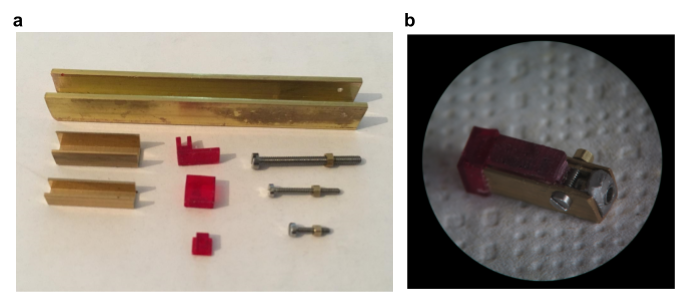
\includegraphics[width=150mm]{figures/F29_microdrive.png}}
\caption[Microdrive]{
Pictures of the custom-made microdrive. (a) 3D-printed and pre-cut brass parts, required to build the microdrive. (b) A picture of the assembled microdrive.
}
\label{fig:F29_microdrive}
\end{figure}

In the beginning of the project, I invested time to design the custom microdrive that meets these criteria (Figure 29 a and b). The major parts needed to assemble the microdrive are the U-shaped rails (commercially available), the M1 and M1.4 10mm screws (also commercially available) and the custom designed plastic parts. The Asiga Pico2 3D printer (https://www.asiga.com/) was used to print the plastic parts. The M1 driving screw having 250um height change per full turn allowed for the 31.25um single movement precision when rotated at 1/8 of a turn per adjustment. The total price of the required parts does not exceed 5 euros, the assemble time does not exceed 1 hour if the printed parts are ready. The drive was successfully implanted to 12 gerbils and proved it’s stability during the recordings. Most of the silicon probes were fully recovered after the end of the experiment, although some had to be trashed due to the surgical issues (recording shanks were clogged by cerebro-spinal fluid or some bleeding and the probe was not recoverable).

\subsection{Protecting box}

In contrast to the different designs of the tetrode drives, which are typically cemented to the skull together with the connector and protection for moving parts, the reusable microdrive with the recording device should be placed in a separate protective enclosure, disconnected from the drive itself. The standard procedure is to build this exclosure from copper mesh during the surgery, gradually building the shielding walls with cement. This method requires careful manipulation of the mesh parts with close proximity to the implanted probe and takes a long time, increasing the duration of the surgery and reducing the chances for successful recovery. The availability of high-precision 3D-printing in house allowed to design a custom protective box that can be assembled directly on the head of the animal during the surgery in a matter of a few minutes (figure 30a). The box has the following properties:

\begin{itemize}
    \item it is fast and easy to assemble during the surgery, easy to dismount at the end of the experiment
    \item it has a quickly removable cover for a) adjustments of electrode’s position, and b) changing the type of the cover from the simple protecting cover to the recording cover that has infra-red sensitive markers, required for tracking system
    \item it’s length and width do not exceed 18x18 mm to not interfere with gerbil eyes and ears position
    \item it is lighter than 3g to not exceed 5g of the total implant weight together with the microdrive
    \item it protects the recording device from dust (while animal is in cage) and light (during recording)
    \item it is strong and can last for long time (up to several months)
\end{itemize}

\begin{figure}
\captionsetup{format=plain}
\makebox[\textwidth]{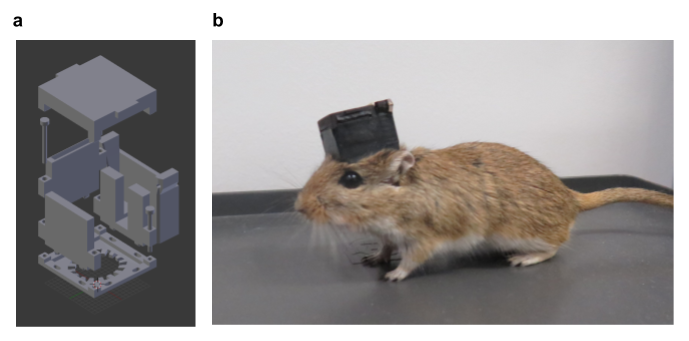
\includegraphics[width=150mm]{figures/F30_crown.png}}
\caption[Protecting box]{
(a) A 3D-model of the protecting box with the connector pocket. (b) A picture of the implant on the animal.
}
\label{fig:F30_crown}
\end{figure}

I designed the corresponding protecting box for 3D printing. I used 1x1.5x5 mm magnets, glued inside both the walls of the box and the top cover, to implement easy access inside for electrode adjustments. The M1 10mm screws were used to hold the walls together. As a result, the overall surgical time decreased and the new implant design allowed for the recovery of the recording device with the connector at the end of the experiment.

The designed protective box was successfully used in 12 animals (figure 30b), 4 of them for the duration of more than 2.5 months. Despite the light accumulation of dust inside the box, due to an imperfect connection between the top cover and the wall with the connector, the box was stable and reliable and didn’t show any failure in all of the animals.


\subsection{Surgery}

Standard stereotaxic surgical procedures of implantation of microelectrodes in the rodent hippocampal area CA1 were performed. Before the surgery, a 3D model prototyping the stages of the implantation was designed to ensure the correct placement of the microdrive and the protecting box, as well as the later fixation of the connector (figure 4.3 a-c). A 3-component solution with medetomidine-midazolam-fentanyl (0.15mg/kg, 7.5mg/kg, 0.03mg/kg) was used to anesthetize animals and keep the anesthesia for the duration of the surgery, by re-injecting the solution every 2 hours if the animal showed foot reflexes. During the surgery, animals were head-fixed in a stereotaxic frame (Stoelting Co.) placed on the heating pad with the termometer to maintain the body temperature of 36°C. All animals were implanted in the right hippocampus. A silicon probe oriented 15\% to the vertical plane attached to a microdrive was inserted into a 2mm wide craniotomy window (AP 3.0mm, ML 3.3mm, DV 0.9mm, averaged using the lambda-bregma distance according to the \cite{Radtke-Schuller2016}). Sealing wax was used to protect the electrodes and to cover the craniotomy window.

\begin{figure}
\captionsetup{format=plain}
\makebox[\textwidth]{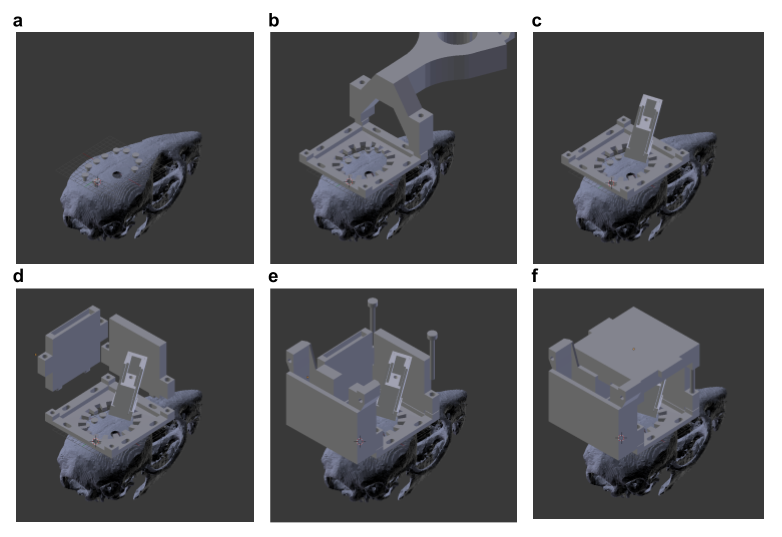
\includegraphics[width=150mm]{figures/F31_surgery.png}}
\caption[Surgical procedures]{
3D-modelled stages of the microdrive insertion and implant assembly during the surgery. (a) Insertion of the grounding screws to the skull. (b) Fixation of the base plate on top of the grounding screws. (c) Placement of the microdrive with the electrodes under the required angle and fixation of the drive with the cement. (d-e) Assembly of the protecting box using M1 10mm screws on top of the base plate. (f) The resulting implant assembled.
}
\label{fig:F31_surgery}
\end{figure}

The base plate, necessary to hold the protecting box, was cemented to the skull together with 10 M1 1mm screws, anchored to the frontal, left parietal and occipital bones (Dental cement, Paladur). Two screws inserted in the occipital bone above the cerebellum served as electrical ground. The surgery finished with the 3-component antagonist atipamezole-flumazenil-naloxone (0.4mg/kg, 0.4mg/kg, 0.5mg/kg). The post-surgical treatment included 5 days of daily injections of antibiotics (Baytril, 10mg/kg) and 3 days of analgesics (meloxicam, 0.2 mg/kg). The recordings started only after complete animal recovery.


\subsection{Recording procedures}

After the successful animal recovery the electrodes were adjusted daily to lower the probe tips with recording channels to the pyramidal layer of hippocampal CA1. Lowering of the electrodes was done in small increments of 1/8 to 1/4 of a turn (31.25 to 62.5um) not exceeding 125um per day to avoid damaging neural tissue and missing the right hippocampal layer. To make a proper adjustment, an animal was connected to the acquisition system before the move of the electrodes and the LFP signal was monitored. The correct placement of the electrodes was defined by several factors, including the presence of sharp waves (\cite{Buzsaki1986}) and ripples (\cite{OKeefe1978}) in the LFP signal during immobility periods, as well as the presence of simultaneous bursts of spikes pointing to the putative pyramidal cell activity in this region. If these factors were not observed within a reasonable time (approx. half an hour) the electrodes were adjusted and an animal was left for another half a day. Otherwise, an experimental session was recorded.


\subsection{Histology}

To confirm the correct electrodes location, a histology on the animal’s brain tissue was performed. Animals were deeply anesthetized with pentobarbital and perfused with 4\% paraformaldehyde. After the perfusion, brains were extracted and stored in paraformaldehyde for at least one day. Brains were sliced coronally in 60um slices and the slices near the craniotomy were stained with neutral red. Pictures of the slices were taken using the 10x microscope (see examples on figure 32).

\begin{figure}
\captionsetup{format=plain}
\makebox[\textwidth]{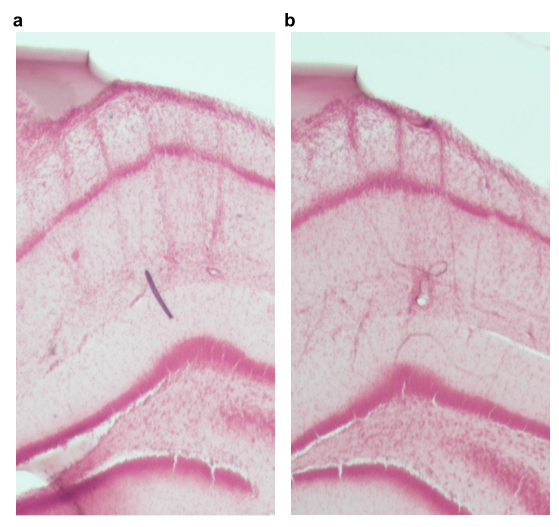
\includegraphics[width=100mm]{figures/F32_histology.png}}
\caption[Histology]{
Example pictures of histological slices. (a) Example picture from animal 00908 slide 6 slice 4 - 2x (b) Example picture from 003281 slide 6 slice 5 - 2x. Note multi-shank tracks of electrodes penetrating the CA1 pyramidal layer (top).
}
\label{fig:F32_histology}
\end{figure}


\section{Virtual reality setup}
\label{sec:vr_setup}

\subsection{RatCAVE system}

All experiments were designed to be conducted in a 3D virtual reality setup named ratCAVE (\cite{DelGrosso2018}). The setup consists of a large rectangular arena (floor area 162 cm × 72 cm and walls of 60 cm height, placed with a 70 degrees angle to accommodate the visual projection),a set of 7 infra-red tracking cameras (Prime 13W 240 fps, OptiTrack, NaturalPoint Inc., United States) located above the arena, and a high-frequency projector (Prime 13W 120 fps, OptiTrack, NaturalPoint Inc., United States), used to project a 3D virtual environment on the walls of the arena. Each experimental session a 3D-printed set of three spherical reflective markers was magnetically attached to the head of the animal, on top of the implant to not interfere with the headstage. These markers were tracked in a closed-loop by the cameras  to be able to adjust the projection depending on the animal's position. Blender (https://www.blender.org/) package was used to design the virtual environment and export it to .obj files, used by the custom-written 3D graphics python software (\cite{Grosso2019}) for rendering.

Two standard linear actuators and a bearing rail system were installed below the arena to physically move the arena ialong one coordinate axis. The maximum move was 30cm, limited by the borders of the projection. The actuators were controlled by an arduino with a motor shield, connected via USB / serial port to the computer with the experiment control software.

\begin{figure}
\captionsetup{format=plain}
\makebox[\textwidth]{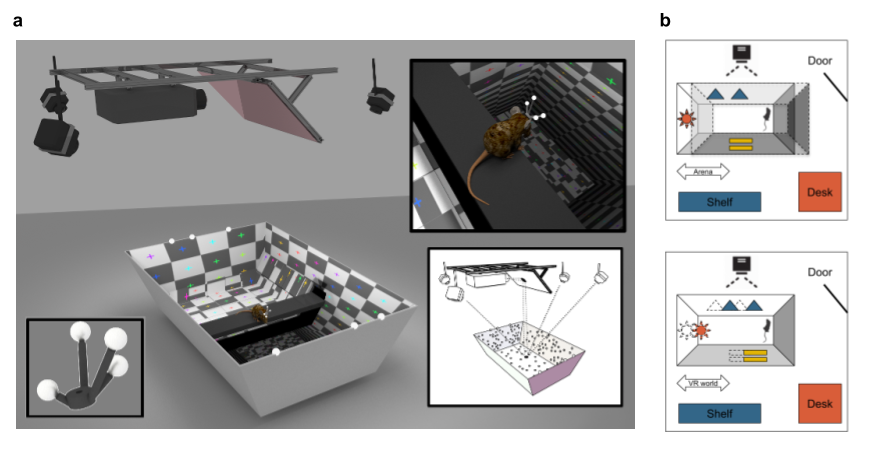
\includegraphics[width=150mm]{figures/F33_VR_setup.png}}
\caption[Virtual Reality Setup]{
The ratCAVE freely-moving virtual reality system for rodents used in experiments. (a) A 3D-model of the arena, position tracking and the projection systems. Left inset (left) shows the reflective markers placed on the animal's head, which is used by the tracking system to locate the animal (adapted from \cite{DelGrosso2018}). (b) Location of the arena in the experimental room and a schematic of the potential experiments: linear translation of the arena using linear actuators (top) or manipulation of the virtual projection (bottom).
}
\label{fig:F33_VR_setup}
\end{figure}


\subsection{Rewarding system}

A food dispenser (Campden Instruments Ltd.), positioned above the arena served for automatic reward administration. As most of the experiments were designed for random foraging, a food dispenser was triggered for dropping a food pellet (20 mg, TestDiet LabTab AIN-76A) at a random location within the arena at 1 minute intervals.


\subsection{Acquisition system}

An Open Ephys acquisition system (www.open-ephys.org , \cite{Siegle2017}) driven by an Opal Kelly XEM-6310 FPGA module was used to acquire neuronal data at a 30kHz sampling rate. The 32 or 64-channel Buzsaki H64 silicon probes were connected via the Intan RHD2000 series headstage to the acquisition box, which transmitted the raw data to the Open Ephys GUI for saving and visualization. The synchronization between the electrophysiology and virtual reality systems was done using the “Network Events” plugin, essentially implemented by periodic sending of TCP packets using python ZeroMQ package from the VR computer to the Open Ephys acquisition socket on the Ephys computer, connected directly via ethernet cable.


\subsection{Automatic experiment control}

A custom experimental control software was written to asynchronously manage the virtual projection, information from the tracking system, linear actuators, food dispenser, visualization of the animal position, video- and position logging and synchronization with the acquisition system. The non-blocking transmission of the information between components was implemented using the PUB/SUB communication scheme based on the ZeroMQ messaging system (https://zeromq.org/). Rendering of the virtual projection was performed by the ratCAVE package (\cite{Grosso2019}), food dispenser and linear actuators were connected and operated via USB serial ports, OpenCV (https://opencv.org/) was used for both video recording and animal position visualization, and built-in python components for metadata and logging.


\section{Data analysis}

Data analysis was primarily done in Python 3.5 with the standard math packages numpy and scipy, as well as scikit-learn, matplotlib and other utility packages. Partially the analysis was done in Matlab R2018b using standard libraries (detection of local minima, detection of center of mass of place fields). Significant amount of analysis was written in Jupyter notebooks for better visualisation. Analysis scripts, jupyter notebooks and the code implementing the data processing workflow are available in the project repository.


\subsection{Data processing workflow}

To increase efficiency and consistency working with large amounts of heterogeneous neuroscience data I developed a custom software automating the data processing workflow. A python package named “stapler” (https://gitlab.lrz.de/asobolev/stapler) was written to implement a pipeline consisting of the following steps:
\begin{itemize}
    \item collecting recording session data about animal positioning, animal electrophysiology and session configuration from the local PCs to the central storage
    \item merging corresponding data into a single folder
    \item converting OpenEphys files to binary formats, creating LFP files, compressing video files
    \item running spike sorting workflow on the raw data (high pass filtering, extracting spikes, PCA on spikes, running KlustaKwik, cleaning up)
    \item backing up unit clusters, syncing position and unit firing data, saving optimized data to HDF5
    \item performing post-processing steps required for final analysis (building place fields, calculate unit metrics, computing center of masses of place fields, running bootstrapping on the spiking data, running density based clustering, calculating place field shift matrixes, creating place field figures for every epoch)
\end{itemize}

The program allowed to change the running configuration for each step independently, enabling having custom processing parameters for different types of experimental sessions.


\subsection{Identification of single units}

Klusta (https://github.com/klusta-team/) software was used to perform spike clustering. The NeuroSuite (http://neurosuite.sourceforge.net/) was used to visualize raw data and to manually filter out noise clusters, as well as to merge similar clusters according to their burstiness and waveform shapes on corresponding channels. Clusters, representing interneurons by their spike width and average firing rate, were not taken into further analysis.
I used cluster isolation distance as a parameter to assess spike sorting quality (\cite{SCHMITZERTORBERT20051}). Clusters having isolation distance < 15 were excluded from further analysis.

\begin{figure}
\captionsetup{format=plain}
\makebox[\textwidth]{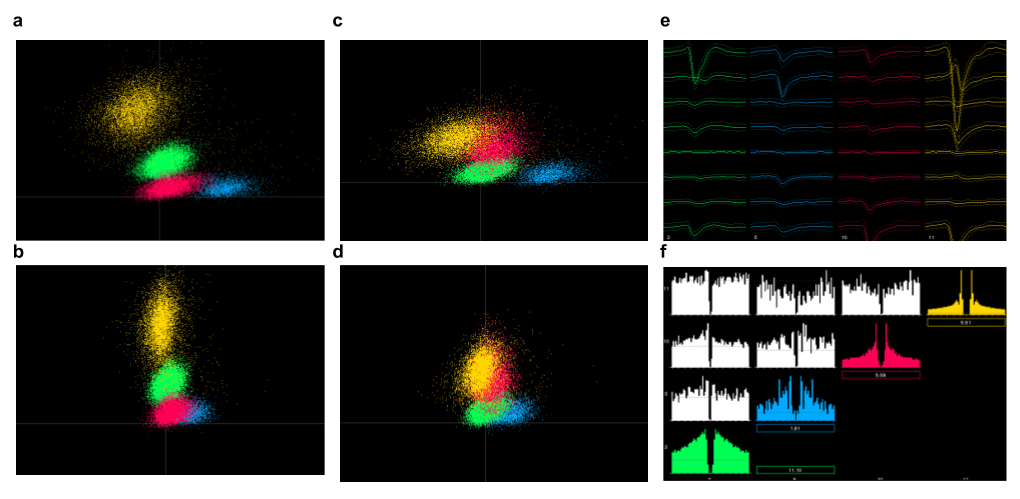
\includegraphics[width=150mm]{figures/F34_spikesorting.png}}
\caption[Spikesorting]{
Spike clustering. (a-d) Example cluster projections in pairs of principal components. Spike belonging to the same cell share the same color. (e) Example waveforms (mean) and (f) cross-correlograms of spiking of the same cells as in (a-d).
}
\label{fig:F34_spikesorting}
\end{figure}


\subsection{Spatial firing maps and place fields}

For every recording session and subsequent experimental condition I calculated spatial firing maps, mainly to visualize the conditional spatial selectivity - the change of the unit firing rate depending on the animal’s and arena position. The space was binned in 0.5 x 0.5 cm squares and the number of spikes for each bin was accumulated. The spiking map was computed by dividing the number of spikes in each square bin by the total time spent in the bin. The resulting firing rate maps were created by applying smoothing with 2D gaussian filter with sigma = 3 cm.

To define the precise analytical locations of place fields, I calculated the areas above the 0.5 * peak firing rate (threshold) of each firing rate map, and each connected area was taken as a putative place field. For each place field the center of mass (COM, Cx; Cy) was calculated:

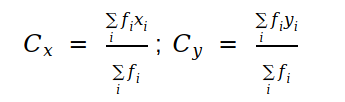
\includegraphics[width=70mm]{assets/formula.png}

where fi  is the firing rate and xi  yi  are the coordinates of the spatial bin. For each place field these centers of masses were not used as a final location of the field but used to further refine the position by bootstrapping.

To reach better precision on defining the place field locations, as well as to exclude noisy fields I used bootstrapping on the original spiking data. First, I split each spike train into several experimental conditions. For each condition I bin the timelapse of the spike train in chunks of 10-15 s and build a new spike train by randomly taking chunks with replacement. As a result of performing this operation 1000 times I get 1000 re-sampled place fields for each experimental condition. Second, for each new re-sampled spike train I compute individual place field locations using the thresholding / center-of-mass method, described above. This resulted in the number of bootstrapped locations of putative place field centers for each unit / condition. By design of the bootstrapping method, the centers of these individual fields tend to cluster together across all resamples if the field is stable, and tend to spread if the field is just noise. To get the actual fields, I used density-based spatial clustering with noise to separate well-connected clusters of bootstrapped field centers. The density-based clustering procedure allows to ignore noisy resamples (less than 100 field centers in the cluster from 1000 resamples), as well as to rank resulting clusters by the number of points (field centers) in the cluster. By taking the clusters with the highest rank I separate the most stable fields from the ones that hardly survive bootstrapping (practically I take the best 2 clusters, e.g taking 2 fields per unit maximum). Finally, the center of each cluster given by the density-based clustering was taken as a final place field location (figure 34 a-c).

\begin{figure}
\captionsetup{format=plain}
\makebox[\textwidth]{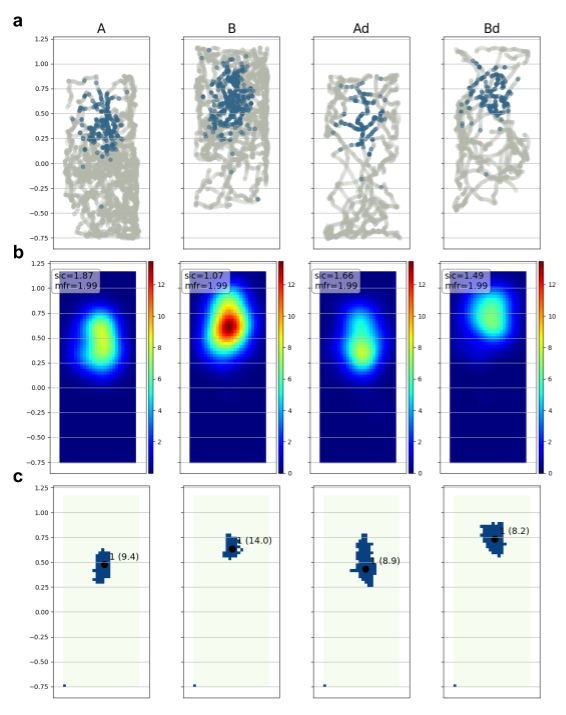
\includegraphics[width=100mm]{figures/F35_place_fields.png}}
\caption[Place field detection]{
Detection of place fields. (a) Example spiking (blue) and arena occupancy (grey) plotted in the arena coordinates. (b) Example firing rate maps of a neuron in (a). (c) Place field patches and their center-of-masses computed using the bootstrapped procedure
}
\label{fig:F35_place_fields}
\end{figure}


\subsection{Place field shift detection}

For each cluster I use it's surface projection to calculate corresponding fields between experimental conditions (Figure 35c). By gradually shifting one projection relative to another in a range from 0 to 0.3 m (the shift of the arena or the virtual projection in all experiments) and computing the maximum of their overlap I determined the clusters which projections overlap the most (if a field in A does not overlap with any other field in B it means it remapped). After the fields are "paired" between conditions the vertical difference between the centers of their clusters (literally center-of-mass of their bootstrapped field centers) is computed as a shift of that particular field between given conditions (Figure 36).

\begin{figure}
\captionsetup{format=plain}
\makebox[\textwidth]{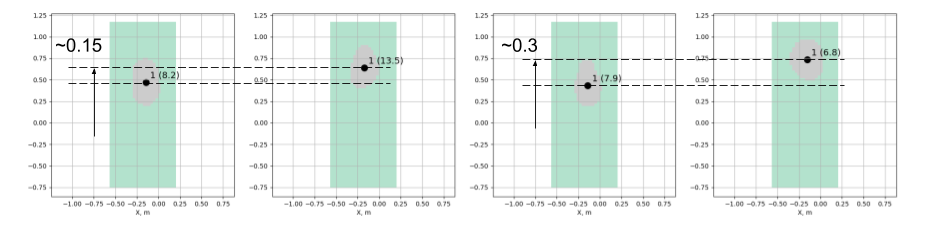
\includegraphics[width=150mm]{figures/F36_shift_detection.png}}
\caption[Field shift detection]{
Detecting place field shift. An example place field with patches in all experimental conditions. This example has only one place field, it has a shift along the Y-axis of 0.15m (light condition, left two plots) and a shift of 0.3m (dark, right two plots).
}
\label{fig:F36_shift_detection}
\end{figure}


%\chapter{Bio2BEL}
\label{ch:bio2bel}

\section{Background on Bio2RDF}

An outline was proposed as early as 1995 for integrating data in the biomedical domain that involved transforming data into a common model, aligning semantically related objects, integrating schemata, and federating data \cite{Davidson1995}. \ac{RDF} has the faculty to address these concerns, and were ultimately realized with the Bio2RDF project, in which multiple biological databases and knowledge bases were serialized to RDF for later integration \cite{Belleau2008}.

As stated before, the expressive power of RDF is counteracted by its lack of domain specificity. While it can be used as an interchange format, it still requires converters to formats for which analytical pipelines have already been developed. Furthermore, the suite of conversion scripts are written in PHP, which has very little traction in the bioinformatics community and therefore is difficult to integrate in pre-existing workflows. This section presents Bio2BEL: a project similar to Bio2RDF for the BEL community to directly the usage of the other tools presented in this thesis.

\section{Generation of Namespace Resources}

There are multiple granularities at which a terminology can be modeled. At the lowest is a vocabulary, in which each term is enumerated and described. Higher is a taxonomy, in which hierarchical relations are expressed. At the highest granularity is an ontology, which contains arbitrary and complex relations.

While it is not the primary goal of knowledge modeling, ontologies can also represent cross-references that connect multiple terminologies that describe the same entities. The most common model for representing ontologies is \ac{OWL} which most commonly uses \ac{RDF} as an interchange format, whose main goal is to provide a platform for semantic integration. This immediately provides ontologies with the facilities developed to support semantic data integration. This is very important in the biomedical domain as rapidly progressing technology frequently results in new experiments and new language for describing biological phenomena.

OWL, and a more domain-specific variant, \ac{OBO}, have been widely adopted by the biomedical domain to structure terminologies and enable semantic integration across knowledge and data sources \cite{Smith2007}. Multiple tools for storing, disseminating, and searching them have been including the Brenda Ontology Explorer \cite{brendaontologyexplorer}, BioPortal \cite{Whetzel2011}, OBO Foundry \cite{Smith2007}, and the EBI \ac{OLS} \cite{Cote2006}.

The semantics of the \ac{BEL} require entities to be identified with a name linked to a namespace. The original framework for handling \ac{BEL} Scripts also provided scripts for gathering different resources (vocabularies, taxonomies, and ontologies) in varying formats and assembling them in a specific namespace file format. One of the advantages of BEL over other systems biology modeling languages is its ability to model knowledge across modes and scales. As it is used to describe new phenotypes, such as the domain of psychiatry, new namespaces must be identified and formatted. Below, two approaches for building new namespaces are described.

\subsection{Direct Generation of Namespace Resources}

The OpenBEL Consortium distributed several scripts that included directives and parsers for acquiring data from multiple knowledge bases and databases and structuring them to BEL namespaces in a reproducible manner. Often, this is necessary to acquire identifiers that are not exported to a standard format like OWL or OBO. Additional scripts were written to improve the reliability of these generators and to convert new namespaces summarized in Table 4.

\begin{table}
\centering
\caption[Direct Namespace Generation]{Data sources for which reusable BEL namespace conversion scripts have been implemented}
\label{tab:direct_namespace_generation}
\def\arraystretch{1.2}
\begin{tabular}{p{5cm} p{10cm}}
Data Source & Description \\
\hline
FlyBase & Drosophila genes and gene products \\
HGNC & Human genes and gene products \\
HGNC Gene Families & Human gene families \\
InterPro & Protein families, domains, and binding sites \\
ChEBML & Experiments describing the effects of chemicals on proteins \\
MeSH Psychiatry and Psychology & A taxonomy of concepts from psychiatry and psychology  \\
dbSNP & \ac{SNP}s \\
miRBase & Premature and mature \ac{miRNA} sequences
\end{tabular}
\end{table}

\subsection{Indirect Generation of Namespace Resources}

BEL namespaces are not generally useful for curators or text-mining platforms to perform named entity recognition. The data sources from which BEL namespaces can be derived often have other rich information (synonyms, hierarchies, and cross-references) that could be structured into an ontology that is more generally useful. 

Some of the namespaces that were originally generated directly by the OpenBEL Framework are derived from ontologies. Since the development of this pipeline, the aforementioned services for hosting ontologies have gained popularity. The \ac{OLS} provides a programmatic \ac{API} from which the terms in a given ontology can be accessed. The source code for this service is available and can be hosted locally. 

The indirect approach uses data sources to build ontologies that can be hosted in \ac{OLS} then to use the \ac{OLS} \ac{API} to iterate over the terms' labels in order to easily convert any ontology to a BEL namespace with a reusable procedure. Already, namespaces in Table 5 have been generated from the publicly available \ac{OLS}. 

\begin{table}
\centering
\caption[OLS-Mediated Namespace Generation]{Ontologies deployed in the OLS from which BEL namespaces have been generated.}
\label{tab:indirect_namespace_generation}
\def\arraystretch{1.2}
\begin{tabular}{p{6cm} p{8cm}}
Ontology & Description \\
\hline
Human Phenotype Ontology & Clinical and phenotypic abnormalities \\
Uber Anatomy Ontology & Anatomical structures in animals
\end{tabular}
\end{table}

As a proof of concept, the data sources in Table 6 have been downloaded and converted to an ontology, deployed on a local \ac{OLS} instance, and converted indirectly to a BEL namespace.

\begin{table}
\centering
\caption[Indirect Namespace Generation]{Data sources from which ontologies have been generated, deployed, and used to generate BEL namespaces.}
\label{tab:indirect_ols_namespace_generation}
\def\arraystretch{1.5}
\begin{tabular}{p{6cm} p{8cm}}
Data Source & Description \\
\hline
\ac{UniProt} & Proteins \\
miRBase & Premature and mature \ac{miRNA} sequences
\end{tabular}
\end{table}

\subsection{Distribution of Namespace Resources}

Each method for downloading, parsing, and generating a namespace is stored as its own self-contained Python package. They share common methods for interacting with the \ac{OLS} in the \verb|ols-client| package. Finally, resources are uniformly deployed and distributed with Artifactory \cite{artifactory}. Common code for uploading to Artifactory is included in PyBEL-Tools. 

\subsection{Discussion Related to Resources}

Not all data sources are amenable to the indirect approach. Infamously, the \ac{MeSH} is a thorough data source that was not developed to accomplish the same goals as ontologies. Therefore, it is incredibly difficult task to map its data to an ontology. Furthermore, the implicit solution to semantic integration that relied on ontologies is not generally applicable. In these scenarios, it is not only necessary to generate a namespace, but also mappings. Previous efforts have relied on lookup tables, but like BEL namespaces, are not generally reusable.

Using ontologies to build namespaces implicitly solves the technical problem of mapping terms from one terminology to another, but this does not necessarily generally solve the biological problem. Mappings between identifiers may have different validity for different applications. While it is often convenient for biological literature to name proteins by their genes' names, this can create ambiguity for genes that produce multiple products in the cases of differential splicing and post-transcriptional modification. For example, in some simplistic domains, it is possible to map HGNC gene identifiers to \ac{UniProt} protein identifiers. However, when modeling complex phenotypes that rely on this mechanism, this mapping cannot be used.

\section{Knowledge Integration}

Knowledge can be represented as statements each consisting of a subject, predicate, and object. As knowledge is assembled, the object of one statement may be the subject of another. This process implicitly builds a knowledge network over which reasoning and inference may be performed. Two general purpose technical solutions for storing statements are relational databases and \ac{RDF}.

A relational database allows for similar statements, often ones with the same types of subjects, same types of objects, and same predicates, to be stored in tables. Each row represents one statement, where the subject and the object are assigned a column and additional columns can represent the metadata associated with the assertion of the statement. While their structure is explicitly, relational databases have the disadvantage of becoming large and complicated when representing many types of knowledge. As a result, many knowledge bases are disparate. Further, the management systems underlying relational databases are generally not amenable to federation.

One solution to this problem is to expose the database through \ac{API}s that can be queried from external services to enable federation of multiple relational databases. A popular solution is the \ac{REST} \ac{API}, but to integrate many data sources might require multiple queries, which can put a strain on technical systems. A newer solution is \ac{GraphQL}, which attempts to provide an abstraction layer between relational databases and \ac{REST} \ac{API}s to handle federation more efficiently.

An alternative medium to relational databases entirely is \ac{RDF}, in which all statements are explicitly stored as triplets of subject, predicate, and object in an alternative database management system called a triple-store. The underlying data can be exposed with a \ac{SPARQL} endpoint, which enables the statements to be queried. Further, it directly enables path queries to enable reasoning and inference. \ac{RDF} was developed to enable federation directly using \ac{SPARQL} endpoints from multiple data sources. It also does not need a well-defined schema in the same way a relational database does. This is both a blessing and a curse; new data can be added quickly, but the lack of structure makes it both technically and pedagogically difficult to make pointed queries.

\subsection{Utility of Biological Expression Language}
Because relational databases and \ac{RDF} are general solution for storing knowledge, they are unaware of the domain-specific needs of knowledge representation and storage in the biomedical domain. Among other modeling languages and formats for systems and networks biology, \ac{BEL} is an apt medium for storing structured knowledge extracted from the literature because it enables inference and reasoning over varying topologies of the resulting networks and also a serialization format for structured knowledge bases to enable integration in a domain-specific medium. It is a solution to overcoming the technical limits imposed by RDF on representing relation metadata and the technical limits imposed by relational databases in constructing and querying networks.

BEL is commonly used for manual curation in a specific disease area. Integrating prior knowledge sources to these networks provides context not only to assist the curator in their understanding of the biological knowledge surrounding their curation, but also allows for automatic enrichment, improved reasoning, and a further step towards building a support system for data interpretation. 

Among the most easily integrable structured knowledge formats in BEL are taxonomies, ontologies, and networks. Taxonomies and ontologies directly provide the facility for reasoning and inferences of new knowledge. Networks, such as bipartite \ac{SNP}-disease, chemical-gene, or gene-pathway networks, can be directly integrated in \ac{BEL}. Even networks created by statistical calculations can be added to \ac{BEL} networks to investigate their explanatory power. For example, the \ac{eSNPO} provides statistical associations between \ac{SNP}s and \ac{GO} biological processes. While these don't have mechanistic support, they can provide additional insight and allow for more informed hypothesis triage in network analysis. Here, two approaches for serializing structured knowledge sources to \ac{BEL} are described.

\subsection{Direct Generation of Knowledge Resources}

While structured, the formats in which knowledge is stored varies by domain. For example, ChEBML \cite{Gaulton2012} is distributed as a relational database, while BKMS-react \cite{Schomburg2017} uses a table with specifically formatted entries to describe reactions. For each source in Table 7, a reusable Python library that downloads, structures, queries, and serializes \ac{BEL} was developed.

\begin{table}
\centering
\caption[Direct Knowledge Resource Generation]{Knowledge bases for which reproducible BEL serialization procedures were implemented.}
\label{tab:direct_knowledge_generation}
\def\arraystretch{1.5}
\begin{tabular}{p{25mm} p{20mm} p{45mm}}
Knowledge Source & Type & Description \\
\hline
ChEMBL & Relational Database & Chemical inhibition and binding of enzymes \\
HGNC Orthologies & Tabular & Gene orthology mappings between human, rat, and mouse \\
BKMS-react & Tabular & Biochemical reactions and catalytic enzymes \\
\ac{eSNPO} & Tabular & Relations between \ac{SNP}s and biological processes
\end{tabular}
\end{table}

\subsection{Indirect Generation of Knowledge Resources}

Serializing knowledge to \ac{BEL} is not generally useful outside of the domain of tools directed towards \ac{BEL} networks.  The knowledge bases from which \ac{BEL} can be derived often have other rich information that is not appropriate for \ac{BEL} that could be structured in other knowledge representation models such as \ac{OWL}. For these cases, the parser and serializer were separated in order to build an intermediate relational database. These have the added benefit of being queryable through \ac{SQL} or exposed with RESTful \ac{API}s for large data sets across networks. Finally, these database schemes have the additional benefit of providing a formalism for the knowledge before serializing it to BEL. As a proof of concept, packages have been developed for the parsing, database storage, and BEL serialization for sources listed in Table 8.

\begin{table}
\centering
\caption[Indirect Knowledge Resource Generation]{Knowledge bases for which an intermediate solution for downloading, parsing, and modeling data were used to facilitate the development of reproducible BEL serialization procedures.}
\label{tab:indirect_knowledge_generation}
\def\arraystretch{1.5}
\begin{tabular}{p{25mm} p{20mm} p{45mm}}
Knowledge Source & Type & Description \\
\hline
Comparative Toxicogenomics Database & \ac{XML} & Relations between chemicals, genes, pathways, and phenotypes \\
InterPro & Hierarchy & Protein Family Hierarchies \\
HGNC Gene Families & Tabular & Gene Family Hierarchies
\end{tabular}
\end{table}

\subsection{Discussion Related to Knowledge Resources}

Many more knowledge bases and data sources exist that could be integrated with \ac{BEL}. For example, \ac{miRNA}-Target interactions stored in mirTarBase \cite{Chou2016} could provide insight to the complex regulation patterns that applies to complex diseases. Other sources of knowledge could be extracted from data-mining pipelines, such as linkage disequilibrium block analysis, gene co-expression analysis, and perturbagen-based differential gene expression analyses to provide additional support to elucidate mechanistic insight from increasingly complicated and large knowledge assemblies.


%\chapter{PyBEL Tools}
\label{ch:pybel_tools}

The following section describes a subset of the functions and workflows that have been developed to assess, enrich, and analyze knowledge assemblies parsed by PyBEL. All code is made available as open source and stored in the PyBEL Tools repository (https://github.com/pybel/pybel-tools) on GitHub. Like PyBEL, it is thoroughly documented as to allow for the community to build upon it.

\section{Critical Assessment of Networks}
Before knowledge assemblies can be used to help interpret data, their validity and robustness must first be quantified. While many dimensions can be explored during this quantification, this section places focus on the identification of biological network motifs that indicate inconsistencies in the knowledge assembly. Network motifs have been studied in the context of transcriptional and phosphorylation networks \cite{Alon2007} and already provide insight to the biological activity. As knowledge networks add the heterogeneity of edges including correlative relationships, many new motifs must be identified and their effects inferred. This section presents the first portions of a taxonomy for network motifs in knowledge assemblies, interpret their effects, and use them assess the \ac{NeuroMMSig} knowledge base.

\subsection{A Taxonomy of Knowledge Assembly Motifs}

The first and most simple motif is a contradictory pair. These occur when there exist multiple edges between a given source and target that have conflicting relations, such as increases vs. decreases. However, contradictory pairs are not canonically invalid. They may arise from the effects of the biological context under which different relations were observed. These cases must be carefully considered.

There are many aspects that can be considered to resolve conflicts that cannot be explained by different biological scenarios. First, the date of publication can be considered. The most recent publication is most likely to have made use of other knowledge available to researchers, and be more right. Alternatively, if many publications were made with conflicting views in a short amount of time, the impact factor of the corresponding citations' journals can be considered.  

While there exists a single motif for identifying contradictory pairs, multiple motifs comprise the set of contradictory triplets. The algorithms that identify these triangles within a network come from a deep graph theoretic background to identify logically inconsistent relations. Because BEL knowledge graphs contain both causal and correlative relations, they can be analyzed jointly. The most simple is a mutually unstable triplet, which occurs when entities A, B, and C all negatively correlate with each other. Similarly, separately unstable triplets occur when A positively correlates with both B and C, but B and C are negatively correlated. Three more triple types are identified where a mix of  correlative and causal relations do not match: increase mismatch triplets, decrease mismatch triplets, and jens triplets.

Alternatively, stability analysis can be conducted to identify elements that are likely to be regulated by other parts of a system. These elements are particularly interesting because of the high impact that any given edge could have that connects to it. There are two types of unstable pairs: chaotic pairs, where A and B both increase each other and dampened pairs, where A and B both decrease each other. The same logic extends to chaotic triplets and dampened triplets. Interestingly, analyses of many knowledge assemblies seldom identified dampened triplets; possibly indicating their biological novelty. Chaotic and dampened cycles of length 4 and above are not identified, because the average number of possible connections at those lengths makes qualitative biological interpretation prohibitively difficult. 

Table 9 presents statistics over the occurrence of various network motifs in the three knowledge assemblies produced during the AETIONOMY project. While each case, such as mutually unstable triples, might be interesting, this provides direct insight into the large amount of effort necessary to investigate each unstable motif and motivates the further development of automated approaches for quantifying the robustness of a given knowledge assembly.

\begin{table}
\centering
\caption[Stability Analysis of NeuroMMSig]{Stability analysis statistics over the AETIONOMY knowledge assemblies for Alzheimer's disease, Parkinson's Disease, and Epilepsy. The ratios suggest that the relative counts of each network motif are not similarly correlated with network size or density. }
\label{tab:stability}
\def\arraystretch{1.5}
\begin{tabular}{p{55mm} p{25mm} p{25mm} p{25mm}}
 & \ac{AD} Knowledge Assembly v4.0.3 & Epilepsy Knowledge Assembly v1.1.2 & \ac{PD} Knowledge Assembly v1.1.1 \\
Chaotic Pairs & 56 & 12 & 16 \\
Chaotic Triples & 115 & 27 & 11 \\
Contradictory Pairs & 68 & 18 & 26 \\
Dampened Pairs & 7 & 2 & 4 \\
Dampened Triples & 1 & 0 & 2 \\
Decrease Mismatch Triples & 20 & 0 & 6 \\
Increase Mismatch Triples & 51 & 4 & 20 \\
Jens Unstable Triples & 657 & 153 & 85 \\
Mutually Unstable Triples & 2 & 0 & 7 \\
Regulatory Pairs & 19 & 9 & 15 \\
Separately Unstable Triples & 16 & 0 & 16
\end{tabular}
\end{table}

\subsection{Discussion}

As data integration projects like Bio2BEL make more data accessible during analysis, further plausibility and stability checks can be performed. One would be to integrate the data from \ac{UniProt} for each function and traverse the Gene Ontology molecular function annotations to identify properly annotated activities and flag improperly annotated ones to be either proposed as new, or fixed. Another example would be to check that protein and gene modifications are annotated properly using \ac{UniProt} and dbSNP, respectively. Adding additional checks using prior knowledge makes \ac{BEL} curation much more accessible to curators with less biological knowledge and also text mining systems that currently have less biological intuition.

\section{Survey of Algorithms}

Algorithms for analyzing pathways and networks can be categorized into three main categories: \ac{ORA}, \ac{FCS}, and \ac{PT} \cite{Khatri2012}. Over-representation analysis often focuses on the number of differentially expressed genes present or absent in a gene set compared to chance, while functional class scoring is less susceptible to large effects and considers the aggregate of groups of small effects. Pathway topology finally considers the biological relations between members of the pathway during analysis.

Furthermore, there is a distinction between methods that rely on the assumption that protein activities are correlated with their corresponding \ac{mRNA}s' expression changes (forward reasoning) versus the effect that upstream controllers of \ac{mRNA} expression have (backwards reasoning) \cite{Martin2014}

These algorithms have been developed for a wide variety of applications, data formats, and graph types. While many are heterogeneous, below are the most notable algorithms specific to networks from knowledge assemblies encoded in \ac{BEL}.

\subsection{Reverse Causal Reasoning}

Reverse causal reasoning (\ac{RCR}) is an approach to identify the upstream controllers of biological patterns measured in an experiment; often differential gene expression experiments between healthy and diseased patients. First, large knowledge assemblies are dissected into smaller hypothesis networks with one upstream node with multiple outgoing causal relations to target nodes represented by the experimental data set. Each hypothesis network is scored by its concordance between the observed up- and down-regulations of targets nodes to the sign of the causal relation and by its richness, or the explanatory power of the hypothesis network \cite{Catlett2013}. An example hypothesis network is shown in Figure 13.

\begin{figure}
\captionsetup{format=plain}
\makebox[\textwidth]{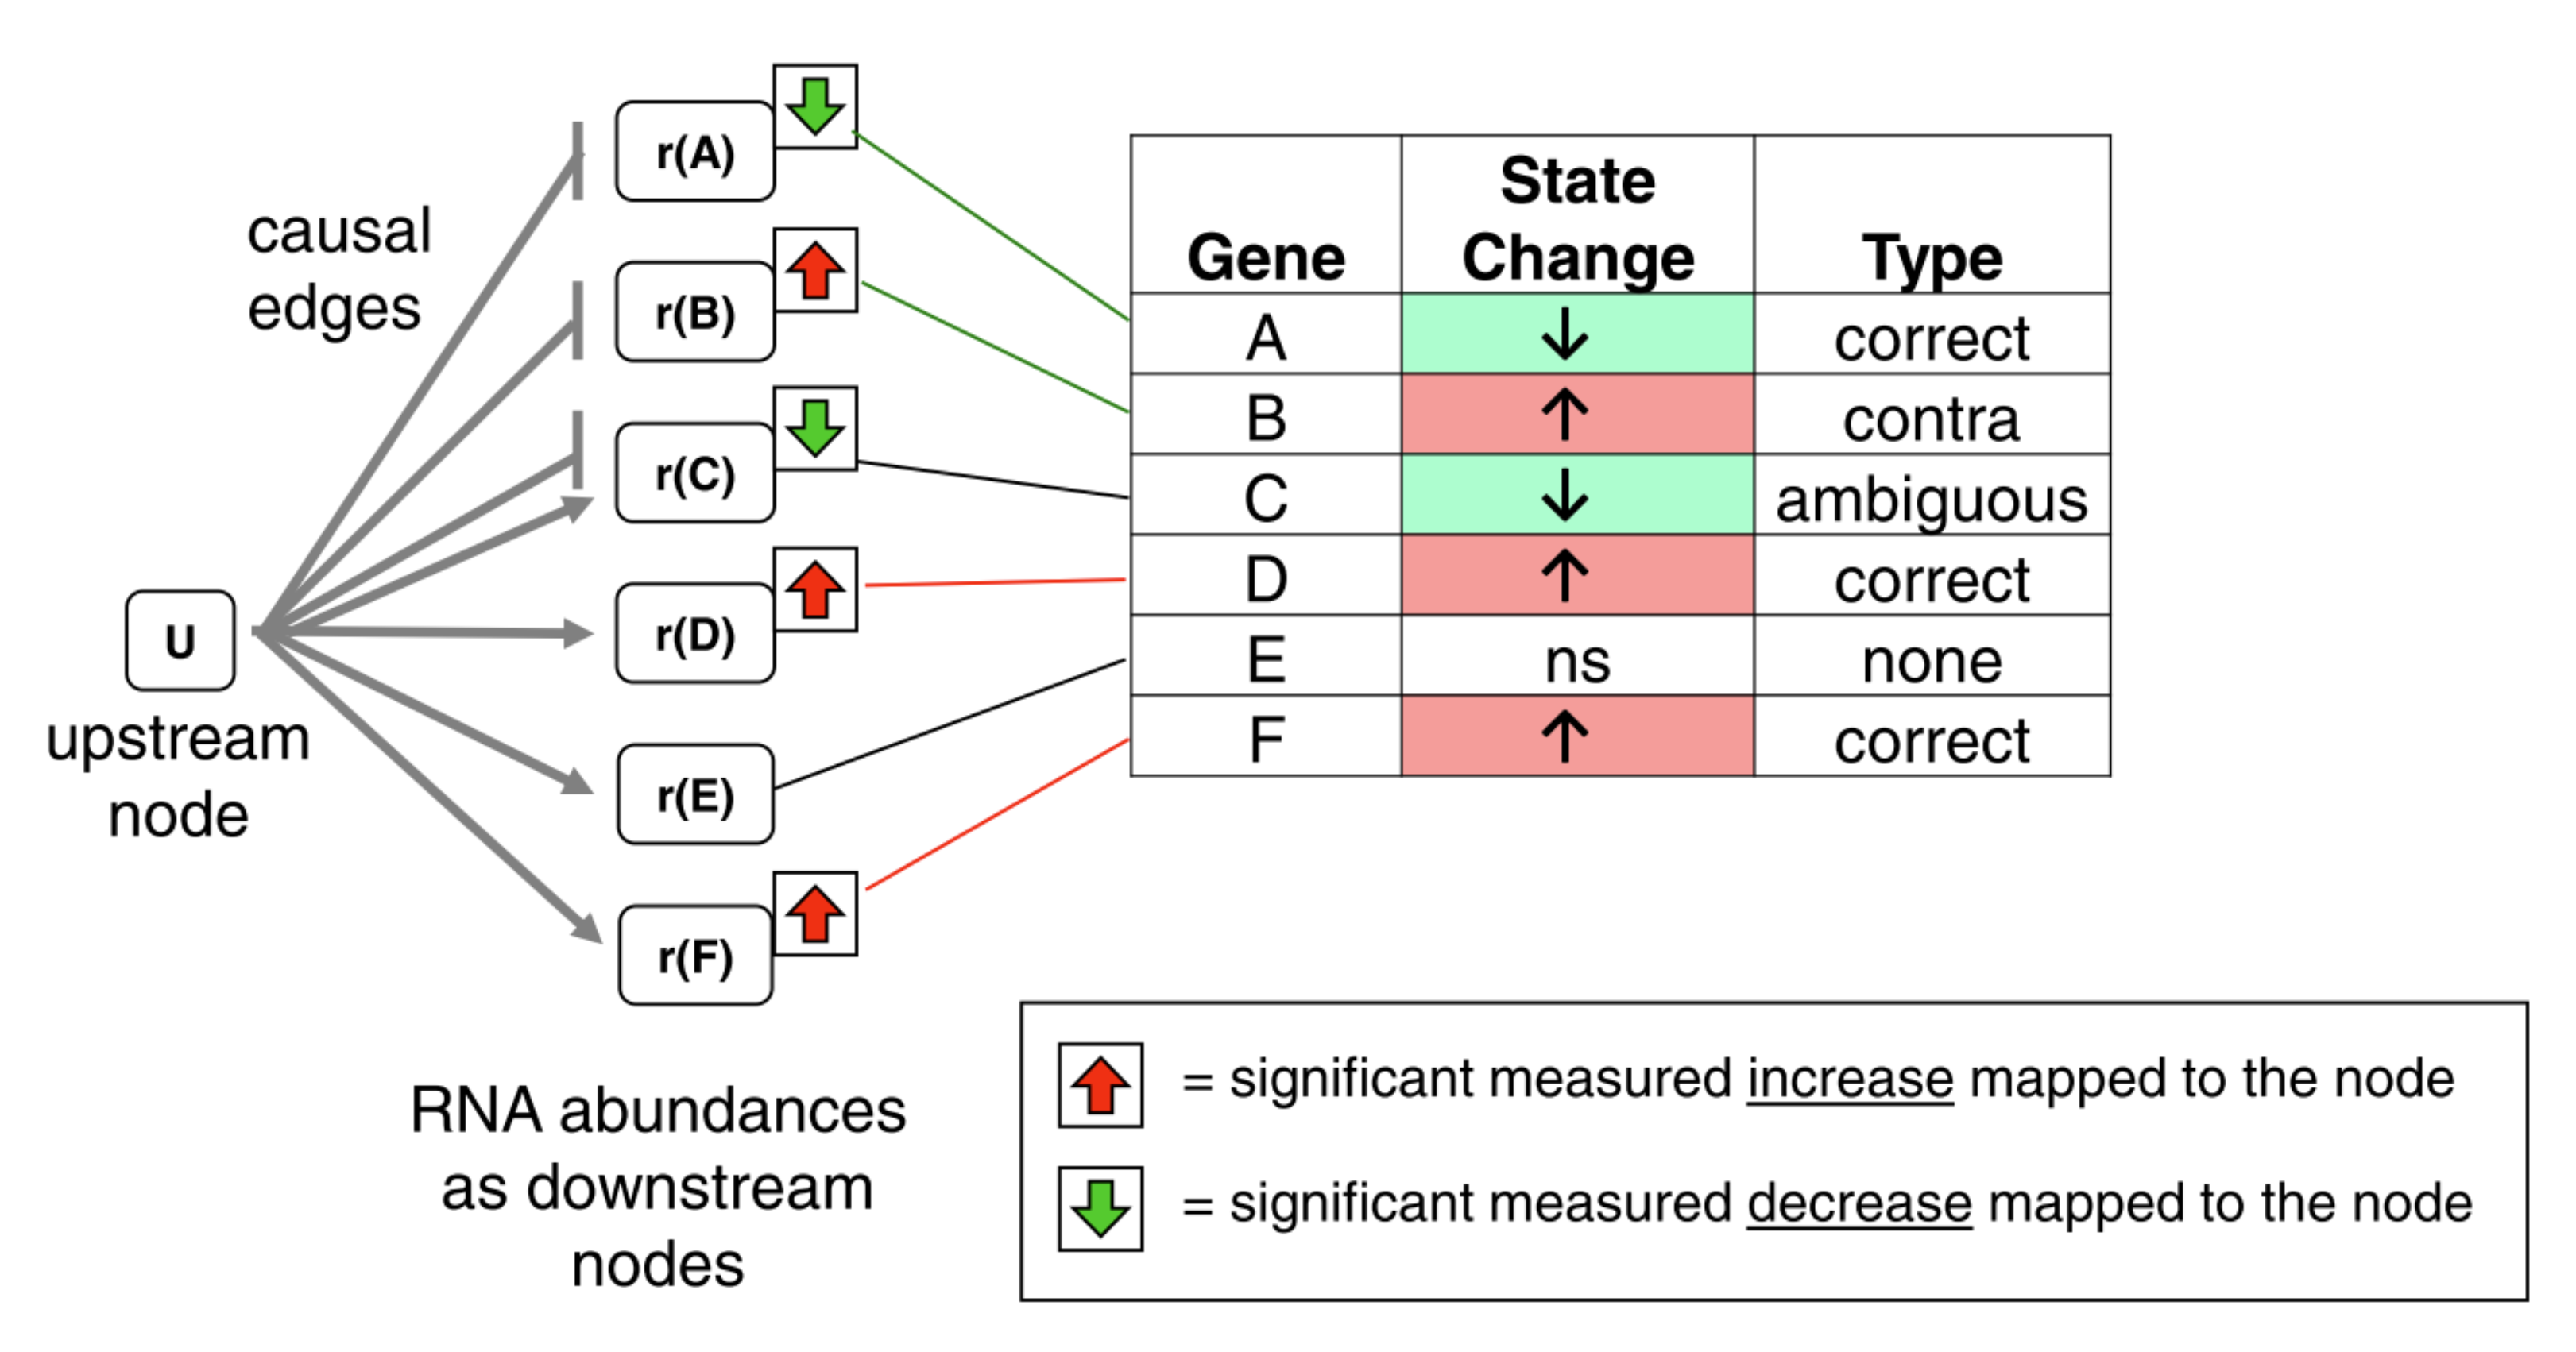
\includegraphics[width=160mm]{images/rcr_schematic.png}}
\caption[A Schematic Diagram of \ac{RCR}]{An example hypothesis network. Target nodes are counted as correct if they have a decreasing relationship and down-regulation, or an increasing relationship and up-regulation. Target nodes with multiple conflicting relationships are marked as ambiguous. Finally, target nodes are counted as incorrect if they have a mismatch between an increasing relationship and down-regulation, or a decreasing relationship and up-regulation. Adapted from \cite{Catlett2013}.}
\label{Fig:rcr_schematic}
\end{figure}

\subsection{Network Perturbation Amplitude}

While \ac{RCR} gives preliminary insights to significant biological controllers, it mostly ignores the topology of signaling, regulatory, and other causal networks that can be represented in knowledge assemblies (Figure 14). The \ac{NPA} measures the aggregated effect explained by the controller layer with reference to a given node with respect to their downstream nodes. Two complementary statistics for the effect of permutations of the upstream layer and downstream layer allow for further insight to the validity of \ac{NPA}s as a hypothesis generation mechanism \cite{Martin2014}.

\begin{figure}
\captionsetup{format=plain}
\makebox[\textwidth]{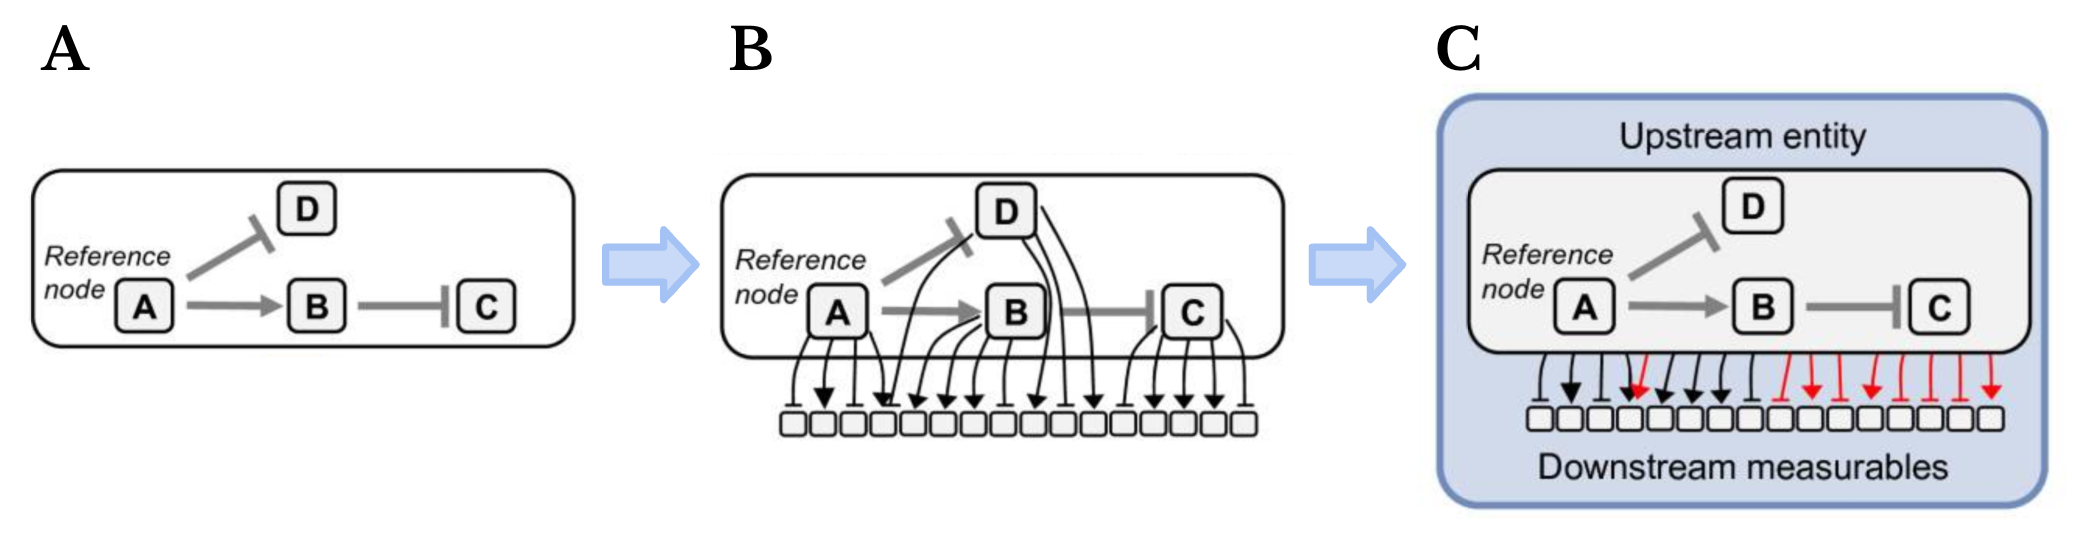
\includegraphics[width=160mm]{images/npa_schematic.png}}
\caption[Hypothesis Network Generation for Network Perturbation Amplitude]{Creation of hypothesis networks that accounts for the topology and interactions of  upstream controller layer with respect to a reference node A), their individual effects on the downstream layer B) and their combine effect C). Adapted from \cite{Martin2012}.}
\label{Fig:npa_schematic}
\end{figure}

\subsection{Sampling of Spanning Trees}

While \ac{NPA} enables more informed analyses than \ac{RCR}, its mathematical basis limits the topologies of knowledge networks that can be used to those with causal consistency. In these networks, all paths from one node to another result in the same aggregated effect of increases and decreases. An additional approach in Figure 15 for \ac{SST} with random walkers eliminates inconsistencies and can be aggregated over multiple trials to assign \ac{NPA} scores to networks that were otherwise inconsistent \cite{Vasilyev2014}. 

\begin{figure}
\captionsetup{format=plain}
\makebox[\textwidth]{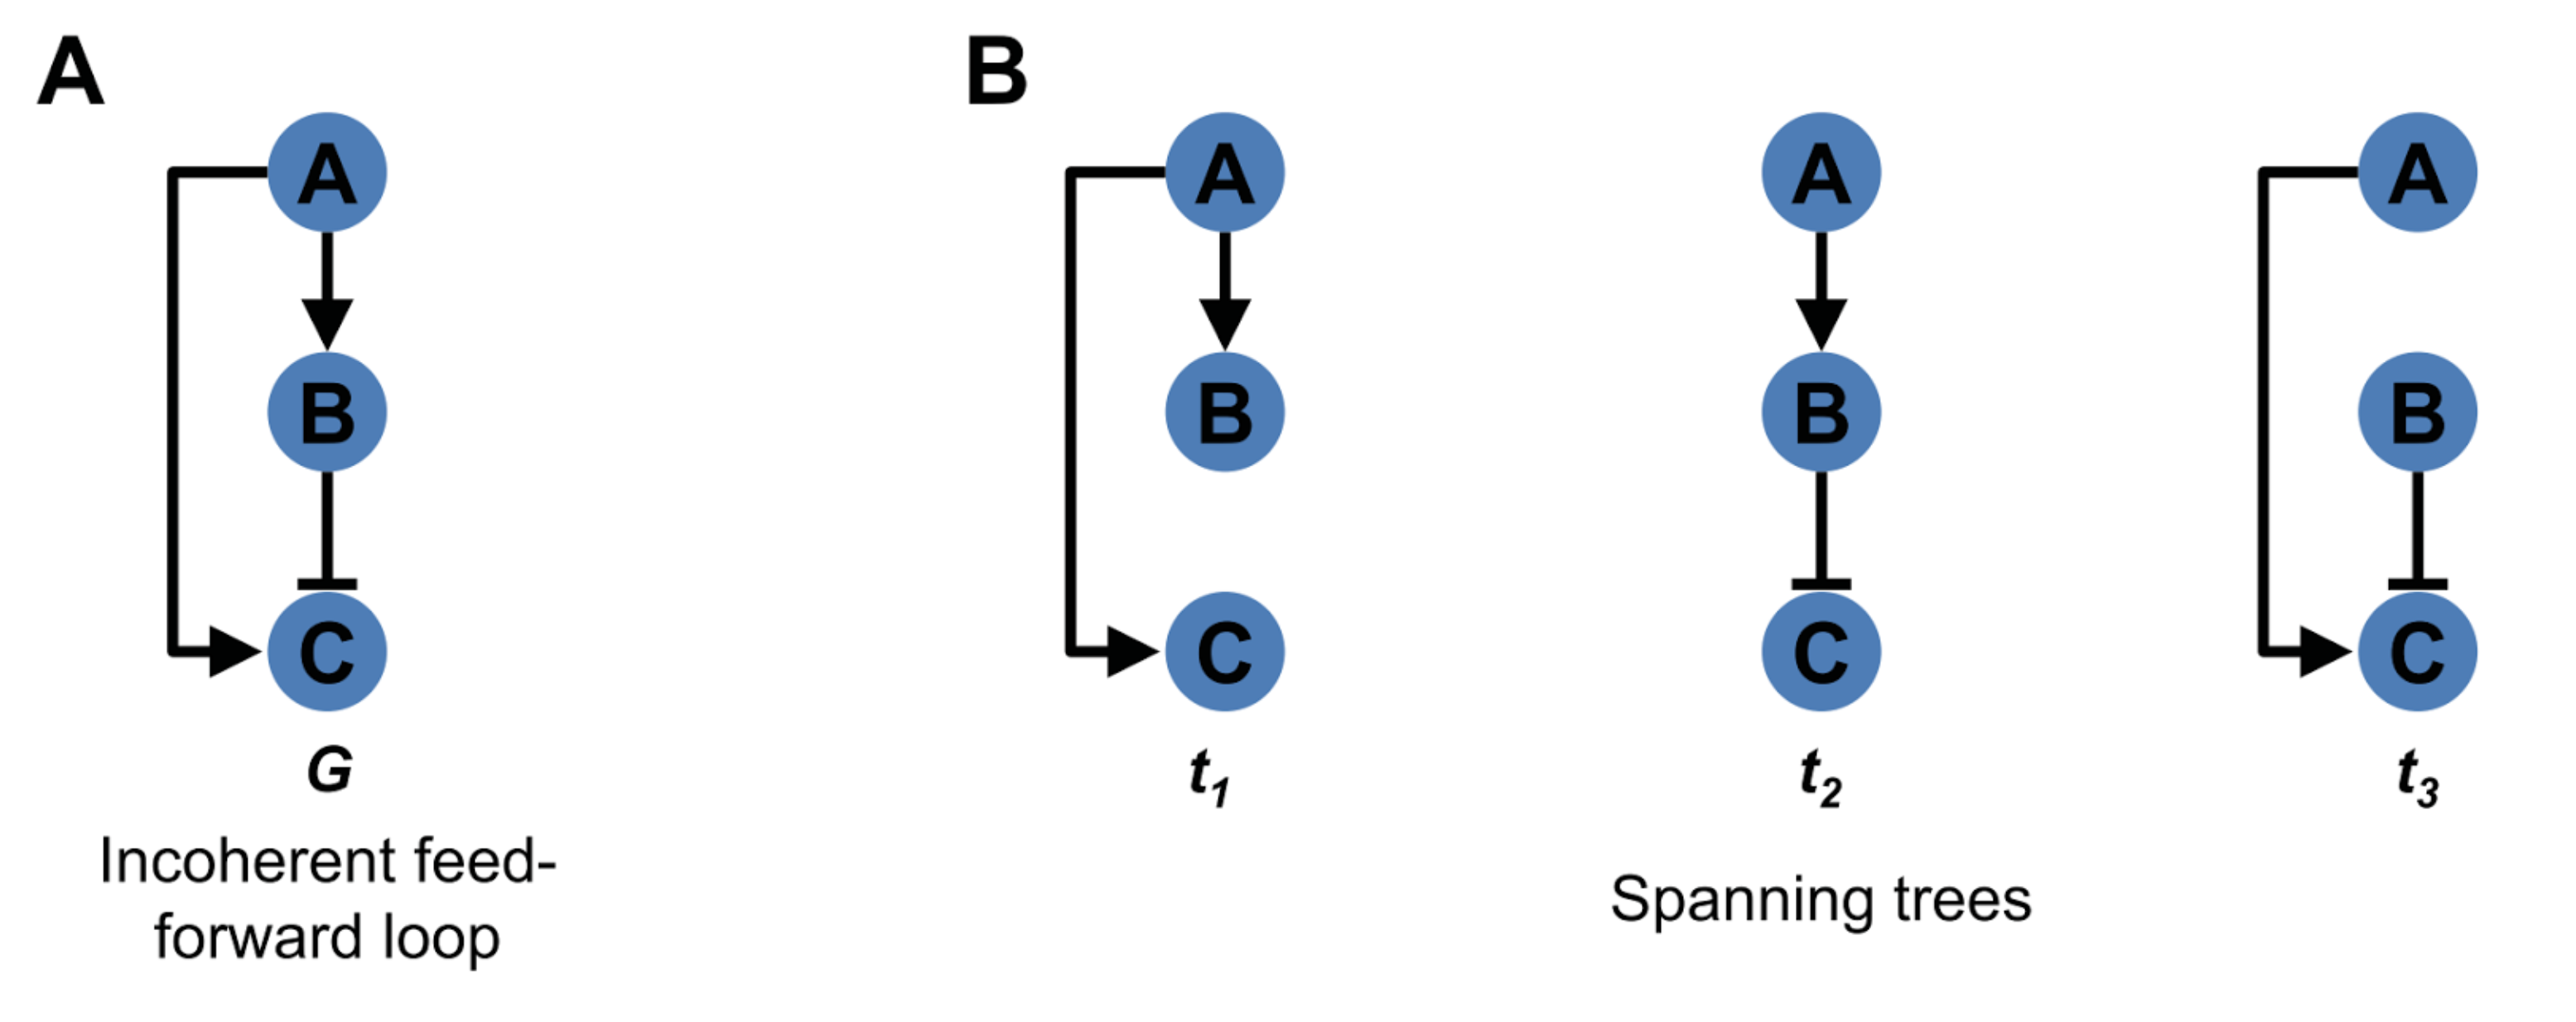
\includegraphics[width=160mm]{images/sst_example.png}}
\caption[Decomposition of Spanning Trees]{An example decomposition of a small causally inconsistent network A) to its spanning trees B)\cite{Vasilyev2014}.}
\label{Fig:sst_schematic}
\end{figure}

\subsection{Unsolved Issues}

While these algorithms already provide significant insight, they still have unresolved issues. For example: they require prior definitions of the upstream controller layer subnetworks; they do not address other exotic network motifs such as contradictions; and they do not take advantage of the vast assembly of correlative relationships. Further, there is generally a low coverage of nodes present in data sets within knowledge assemblies.

As mentioned before, these algorithms were developed for domains (oncology, immunology, etc.) that are rich in molecular data and mechanistic knowledge. For disease areas such as neurodegenerative diseases, molecular data (e.g., microarray, \ac{RNA}-seq) are not often available for the most applicable cells or tissues because of the practical difficulty of acquiring samples. It follows that context-specific knowledge is also much more sparse; and inference from other contexts (such as animal models) is much less reliable.

While backwards reasoning overcomes the issues with interpretation that are posed by forwards reasoning, the insufficient knowledge and data in neurodegenerative diseases makes this revelation much less useful. 

The experimental data available in for this field and other complex diseases are often multi-modal and multi-scale, prompting the development of new methods. Many of these experiments can only be connected to current knowledge assembles through correlative relationships, such as the associations between single nucleotide polymorphisms (\ac{SNP}s) and clinical phenotypes such as neuroimaging and gene expression. 

\section{A Priori Network Augmentation}

This section first describes pipelines that make biological knowledge assemblies more usable that rely on prior knowledge from the biomedical domain. Before developing analytical algorithms, it is first necessary to consider pipelines that improve the features of currently existing networks. After, an algorithm for generating upper layer controller networks is proposed and an alternative heat-diffusion method that is better able to accommodate heterogeneous experimental data. 

\subsection{Connecting Disconnected Components}

The GABA Subgraph in the Alzheimer's disease knowledge assembly has five disconnected components. While these can be inspected manually and the gaps can be filled, this becomes a daunting task for the set of 128 subgraphs in NeuroMMSig. PyBEL can be used to build queries that automatically expand and enrich graphs in order to create an environment in which disparate knowledge can be assembled to elucidate mechanistic understanding. Below, a procedure for filling in the holes in a subgraph is outlined. 

First, the central dogma is inferred. This ensures the existence of the corresponding RNA for proteins, and the corresponding genes for each \ac{RNA} and \ac{miRNA}. Doing so already connects the subgraph containing the relations describing how estradiol affects the expression of GABRA4 and GABR3 \ac{mRNA} \cite{Noriega2010} to another component that describes the functional impact of their translated proteins on other proteins and biological processes. After this process, four components remain.

Next, unqualified edges are enriched. This method reasons over nodes for which assertions can automatically be presumed. Relationships describing the different types of variations on genes and proteins (epigenetics, mutations, and post-translational modifications) are able to connect the GRIN2B node that is important in one large component to the phosphorylated GRIN2B node in another network. Because \ac{BEL} represents knowledge assemblies and not necessarily mechanistic models, these pieces of information can come from multiple curators without mutual knowledge. After this process, two components remain.

Of the two components, there is one large component and one small component, consisting only of cAMP catabolic process and GABBR2. While they are not yet automatic, further knowledge-based approaches can be used to connect GABBR2 to GABBR1 in the large component using resources like \ac{HGNC} Gene Families \cite{Gray2015}, InterPro \cite{Finn2017}, or PFAM \cite{Finn2016}. This is valuable because hierarchical knowledge sources like these can be used to reason over the network, like using the knowledge that GABBR2 decreases the cAMP catabolic process  \cite{Massone2011} to assert that GABBR1, the other member of the GPCR family 3, GABA-B receptor (IPR001828), shares the same activity. While this knowledge does not exist in the assembly, literature search also notes several connections between GABBR1 and cAMP signalling \cite{Frere2004,Palmer2005}.

\subsection{Subgraph Membership Inference}

While connecting components is important, it would also be useful to identify and add edges that should belong to the GABA subgraph but do not already. The first method would be to identify and edges occurring between nodes in the subgraph that are not already present, and add them. Next, this procedure can be continued to identify nodes that have edges to multiple nodes already in the subgraph. To reduce false positives, nodes added this way must both be the target of a causal relationship from a node in the subgraph and also have a causal effect on another node in the subgraph.

Finally, to improve viewability, two additional filters are provided. First, a filter for pathologies is used to remove them. This is useful since most pathologies are "super nodes" in knowledge assemblies and have numerous and often uninformative correlative relationships. Next, the central dogma is collapsed such that genes, \ac{RNA}s, and proteins are all shown as one node. While this limits the mechanistic explanatory power of a visualization, it removes a significant amount of visual clutter. 

\subsection{Pipeline Building}

It may be reasonable for viewing purpose to additionally collapse nodes representing modifications to their reference node as well. The submodule \\ 
\verb|pybel-tools.mutation| contains large library of functions that can be chained together either manually, or with a pipeline builder to promote reusability by allowing uses to save their workflows and reuse them. 

\section{Data Driven Analysis}

\subsection{Unbiased Candidate Mechanism Generation}

There are many terms used to describe portions of biological networks including pathways, mechanisms, subgraphs. They all comprise of individual interactions that accumulate to a more complex function. Often, an interaction may be part of multiple of these features. Knowledge bases like \ac{KEGG}, Reactome, and WikiPathways organize interactions into pathways; but they all suffer from bias in the literature and from the knowledge of their curators. This section presents an algorithm for generating unbiased candidate mechanisms from a given knowledge assembly. The method is then compared to the NeuroMMSig knowledge base to identify its ability to reproduce dogmatic subgraphs and identify areas of the underlying knowledge assemblies that have yet to be annotated.

In biomedical knowledge assembly across scales, biological processes represent entire subnetworks of causal interactions through both time and space. The \ac{NeuroMMSig} knowledge base captures associative, correlative,  and causal relationships between genes and gene products and biological processes directly in BEL. Because biological processes implicitly represent functional subnetworks, they are an appealing starting point for automatically unbiased generating candidate mechanisms to be used by other algorithms. 

The upstream controllers of biological processes provide direct insight to their functional impacts across scales. Therefore, the simple algorithm for generating candidate mechanisms that are unbiased by the dogmatic  takes the causally upstream controllers of a biological process, their upstream controllers, and all internal causal edges between them as a candidate mechanism. This method is thresholded at an expansion of two neighborhoods, but could easily be modified to choose larger or smaller lengths.

\subsection{Comparison to NeuroMMSig Knowledge Base}

This method was applied to the NeuroMMSig Alzheimer's disease knowledge assembly for each biological process. After, the resulting candidate mechanisms are compared to the NeuroMMSig subgraphs. First, the landscape of biological process membership in each subgraph is summarized with Figure 16. 

\begin{figure}
\captionsetup{format=plain}
\makebox[\textwidth]{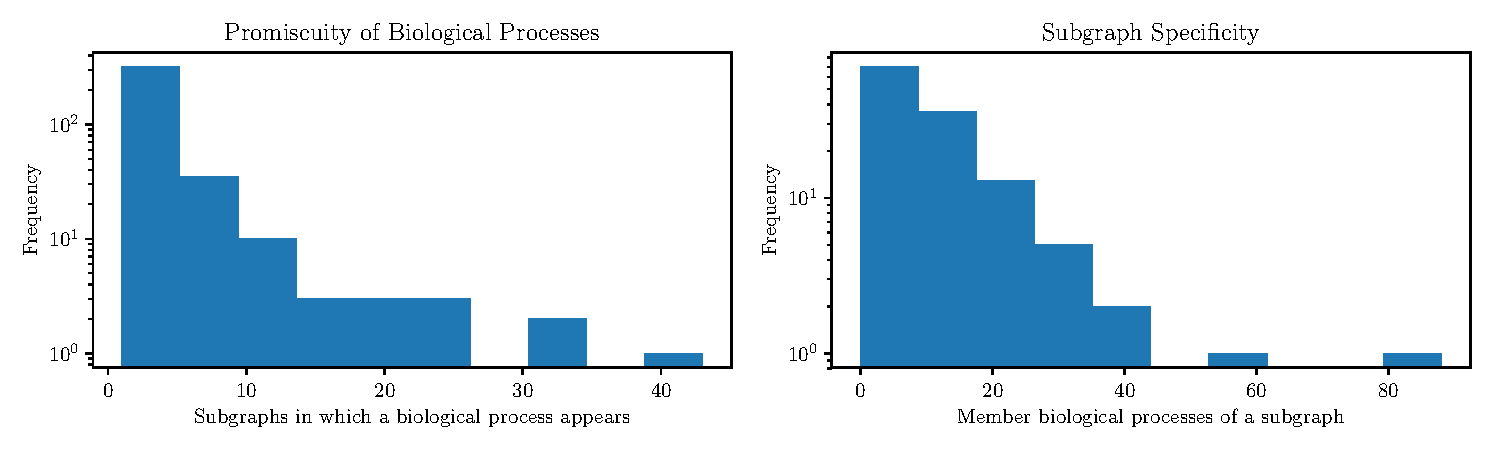
\includegraphics[width=160mm]{images/sg_comparison.pdf}}
\caption[The Landscape of Biological Process Membership in NeuroMMSig Subgraphs]{The landscape of biological process membership shows that there are both biological processes that appear in few and many subgraphs, and subgraphs with few and many biological processes.}
\label{Fig:sg_comparison}
\end{figure}

\begin{figure}
\captionsetup{format=plain}
\makebox[\textwidth]{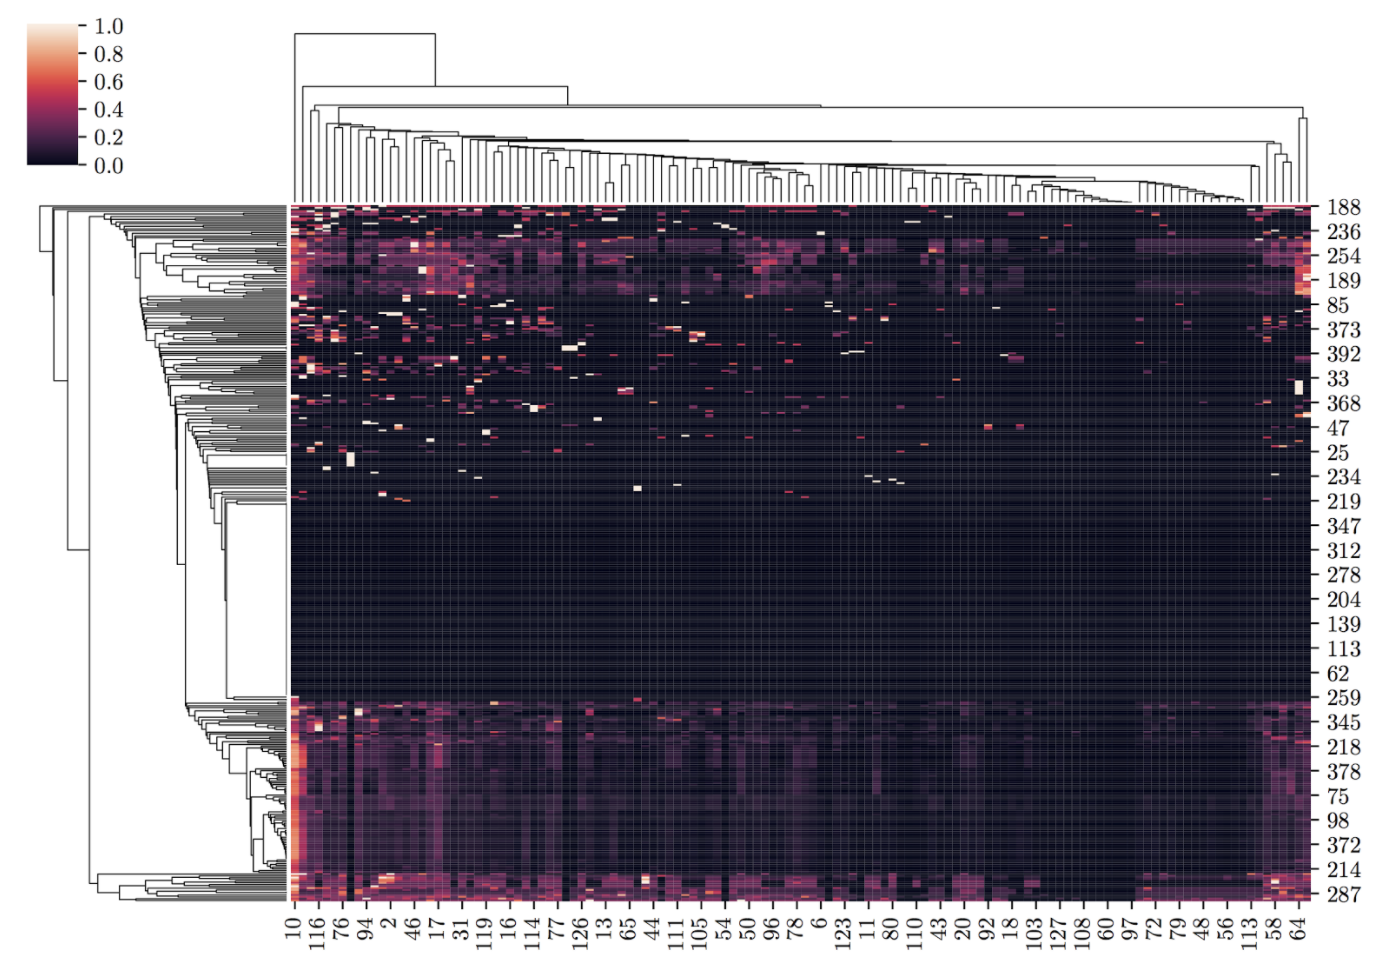
\includegraphics[width=160mm]{images/neurommsig_overlaps.png}}
\caption[Summary of the Overlap of Candidate Mechanisms with NeuroMMSig Subgraphs]{The landscape of candidate mechanism and \ac{NeuroMMSig} overlap, calculated by node overlap. The dark horizontal section directly identifies biological processes that are not annotated in any \ac{NeuroMMSig} subgraphs. This implicates their huge explanatory potential since they are outside the research dogma in Alzheimer's disease research.}
\label{Fig:neurommsig_overlaps}
\end{figure}

This landscape can also be used to annotate new candidate mechanisms to the dogmatic subgraphs in \ac{NeuroMMSig} to allow for more relevant mechanistic analysis. The annotation of further biological processes to subgraphs (Figure 17) can also allow the enrichment strategies in the \ac{NeuroMMSig} Mechanism Enrichment Server to perform enrichment over nodes corresponding to concepts on other scales.

\subsection{Candidate Mechanism Perturbation Amplitude}

All of the previous ideas from this thesis cumulate in the ability to devise and implement an algorithm for data-driven, schema-free analysis of networks. After networks are curated, parsed, enriched, checked for robustness, and triaged into unbiased candidate mechanisms, they can finally be analyzed. This section presents the candidate mechanism perturbation amplitude algorithm. It addresses the issues posed by previous algorithms with more complex randomized approaches and ultimately enables analysis of new modes of data by using a classical schema-free analytical technique similar inspired by other heat diffusion analyses in networks biology \cite{Bernabo2014,Leiserson2015}. The example presented below includes the use of differential gene expression analysis from Alzheimer's disease applied to the unbiased candidate mechanisms generated from the \ac{NeuroMMSig} knowledge assembly.

In this algorithm, heat is applied to the nodes based on the data set. For the differential gene expression experiment, the log-fold-change values were used instead of the corrected p-values to allow for the effects of up- and down-regulation to be admitted in the analysis. Finally, heat diffusion was run with the constraint that decreases edges cause the sign of the heat to be flipped. Because of the construction of unbiased candidate mechanisms, all heat will flow towards their seed biological process nodes. The amount of heat on the biological process node after heat diffusion stops becomes the score for the whole candidate mechanism.

Because heat always flows towards the biological process node, it is possible to remove leaf nodes (nodes with no incoming edges) after each step, since their heat will never change. 

The issue of inconsistent causal networks addressed by the SST algorithm does not affect heat diffusion algorithms since it can quantify multiple conflicting pathways. However, it does not address the possibility of contradictory edges, for example, when A increases B and A decreases B are both true. A random sampling approach is used on networks with contradictory edges and aggregate statistics over multiple trials are used to assess the robustness of the scores as a function of the topology of the underlying candidate mechanisms.

Finally, this algorithm can be tuned to allow the use of correlative relationships. Because many multi-scale and multi-modal data are often measured with correlations to molecular features, this enables experiments to be run using SNP or brain imaging features, whose experiments often measure their correlation with the activity of gene products. 

\subsection{Application Scenario}

This algorithm was applied with the Alzheimer's disease knowledge assembly to assist in interpretation of the differential gene expression experiments from GSE28146 \cite{Blalock2011}. This trial classified patients into three disease progression stages: early, moderate, and severe. While BEL has inherent limits in its temporal expressivity, interpreting data that has an inherent temporal ordering helps overcome this limit. The results for each time point can be accessed at \verb|https://github.com/pybel/pybel-notebooks/blob/master/results/time_series_cmpa.csv|.

\begin{figure}
\captionsetup{format=plain}
\makebox[\textwidth]{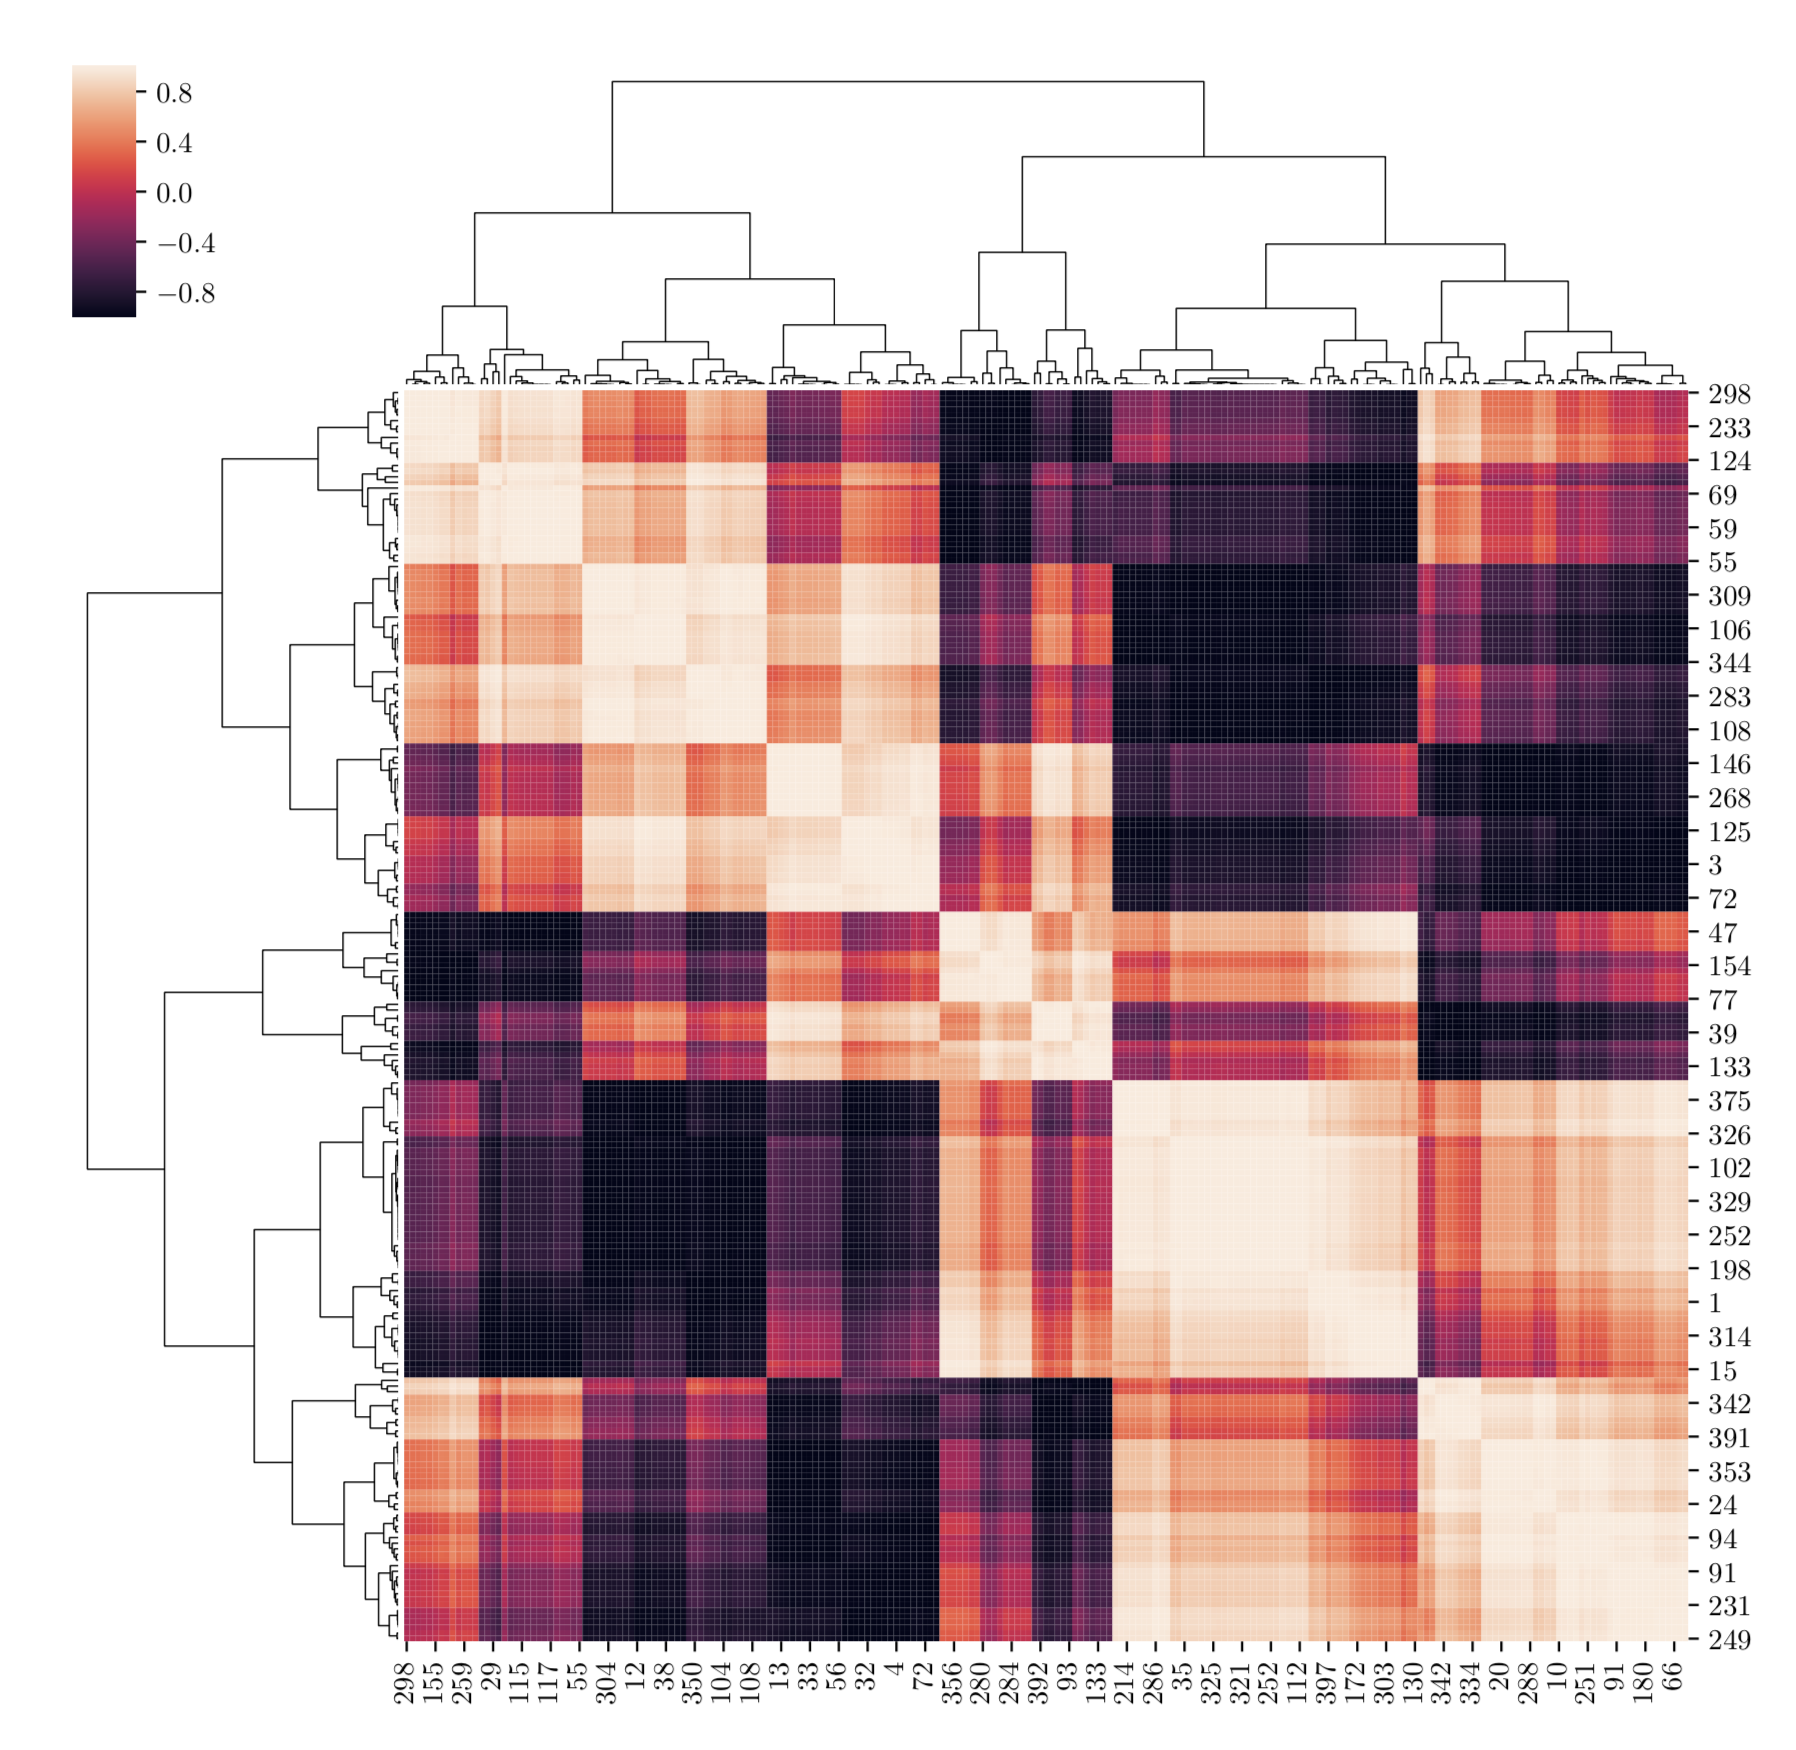
\includegraphics[width=160mm]{images/time_series_clustering.png}}
\caption[Clustering of Time-series Candidate Mechanism Perturbation Amplitude Scores]{A hierarchical clustering over the Pearson correlation of each candidate mechanism score through time suggests there are 4-6 discernible classes.}
\label{Fig:time_series_clustering}
\end{figure}

\begin{figure}
\captionsetup{format=plain}
\makebox[\textwidth]{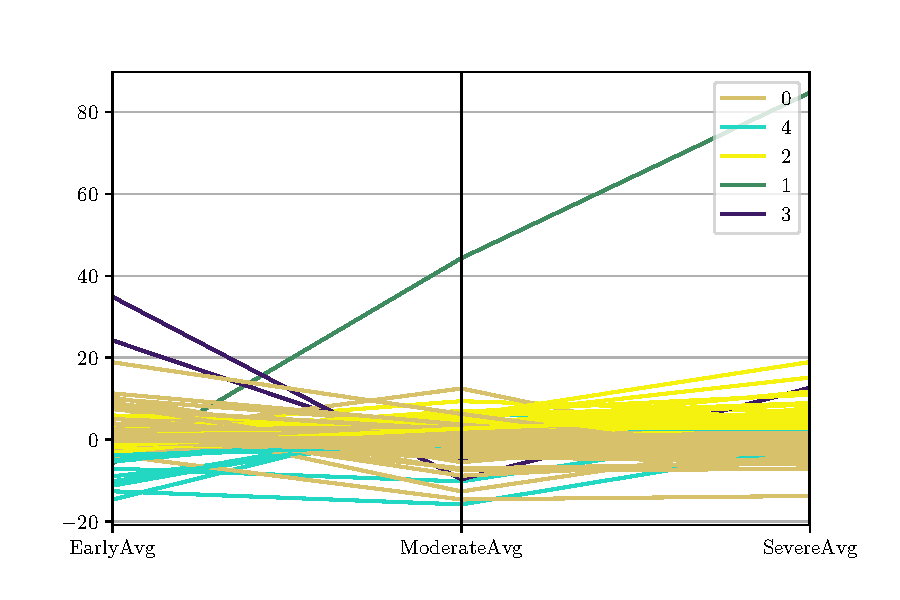
\includegraphics[width=120mm]{images/time_series_pc.pdf}}
\caption[Time-series Candidate Mechanism Perturbation Amplitude Score]{Parallel coordinate plot of all candidate mechanism with coloring by cluster shows the different progressions of biological processes.}
\label{Fig:time_series_pc}
\end{figure}

A hierarchical clustering (Figure 18) was performed using the Pearson correlation coefficient to group biological processes whose observed perturbation changed similarly through time. The dendrogram suggested there were between 4-6 groups of similarly varying processes. In order to make an interpretation, the original values are displayed in a parallel coordinate plot (Figure 19) with colors corresponding to their classes.

In figure 19, class 1 (green) is consists of biological processes that continually increase throughout the progression of the disease. Notably, it contains the inflammatory response. Class 3 (purple) contains biological processes that decrease from the early to moderate stage then increase again. This refers to cell death and neuron death processes. Class 4 includes processes that are initially down-regulated then become less regulated, including mitochondrion-related pathways. Class 2 (yellow) includes processes that do not become disregulated until the severe onset of disease, and have much more variety from glutamate secretion to ion homeostatic processes to metabolic processes. The remaining class does not show significant regulation in any of the disease stages. 

While Alzheimer's disease must be studied with respect to its progression over time, this analysis can provide insight directly to measurements performed on a single time series. Those results provide a ranking that prioritizes the most up- and down-regulated biological processes as a function of the observed data. 


%\chapter{Conclusion and outlook}

This master's thesis was originally motivated by the desire to automatically interpret data sets and generate hypotheses using prior knowledge. While working towards that goal, it was necessary to develop an entire computational infrastructure for BEL. That infrastructure was extended with reusable components to integrate prior knowledge from other sources in order to model biology at the finest granularity possible. Next, a framework for testing the validity and robustness of those knowledge assemblies was implemented and applied to the \ac{NeuroMMSig} knowledge base. Finally, algorithms for extracting meaningful subnetworks were applied to enable schema-free and multi-modal analysis using a heat diffusion algorithm. Using this workflow, it is now possible to interpret multi-modal data sets and generate hypotheses in a truly automated fashion.


\printbibliography

\backmatter

\chapter*{Declaration}
I hereby certify that this material is my own work, that I used only those sources and resources referred to in the thesis, and that I have identified citations as such.

\vspace{0.3in}

\noindent Bonn, \today

\vspace{1in}

\noindent Charles Tapley Hoyt

\end{document}
